\documentclass{article}
\usepackage{geometry}
\usepackage{graphicx} % Required for inserting images
\usepackage{enumitem}
\usepackage{amsmath}

\usepackage{caption}
\usepackage{subcaption}

\usepackage{hyperref}
\hypersetup{
    citecolor = blue,
    colorlinks = true,
    linkcolor = blue,
    urlcolor  = red,
    % linkbordercolor = {white},
}

\usepackage[compat=1.1.0]{tikz-feynman}
\usepackage{tabularx}
\usepackage{wrapfig}

% Uncomment below to check document without figures/tables.
% \usepackage{environ}
% \RenewEnviron{figure}{}% Gobble figure environment
% \RenewEnviron{table}{}% Gobble table environment

\title{Monte Carlo Simulations for Particle Physics}
\author{Victor Manuel Granados Pinto}
\date{August 2024}

\begin{document}

\maketitle

\begin{abstract}
    In this project, a Monte Carlo event generator for the simulation of the process $\mathrm{e}^{+} \mathrm{e}^{-} \to \mathrm{q} \bar{\mathrm{q}}$ has been developed. In the first section, the integration of the cross-section for the fixed-order description of the $2 \to 2$ scattering process at leading order in the Matrix element is discussed. Then, in section 2, the scattering process is supplemented with an all-order simulation of the cascade of bremsstrahlung emitted by the quark-antiquark pair.
\end{abstract}

\tableofcontents

\section{Simulation of the \texorpdfstring{$\mathrm{e}^{+} \mathrm{e}^{-} \to \mathrm{q} \bar{\mathrm{q}}$}{ee -> qqbar} scattering process at fixed-order QED}

For the first part of this project, a Monte Carlo integrator was developed to evaluate the cross-section for the process $\mathrm{e}^{-} \mathrm{e}^{+} \to \mathrm{q} \bar{\mathrm{q}}$ to leading-order. In this section, after a brief introduction to the relevant properties of the differential cross-section to be integrated, the general idea for the Monte Carlo integrator here developed is discussed. Then, some results for the values of the cross-section and their associated error estimates are presented. Finally, as an example of more advanced implementations of Monte Carlo integrators, the \texttt{vegas} package is used to integrate the differential cross-section, for which the results and its algorithm are commented on.

\subsection{The differential cross-section at leading order}

At leading order, the matrix element for the process $\mathrm{e}^{-} \mathrm{e}^{+} \to \mathrm{q} \bar{\mathrm{q}}$ consists of two $s$-channel contributions which differ by having either a photon or a Z boson as the “intermediary” particle, as shown in the Feynman diagram in \autoref{fig:feynman-diagram}.
\begin{figure}[ht!]
    \centering
    \feynmandiagram [horizontal=a to b] {i1 [particle=\(\mathrm{e}^{+}\)] -- [anti fermion] a -- [anti fermion] i2 [particle=\(\mathrm{e}^{-}\)], a -- [photon, edge label={\(\gamma\), $\mathrm{Z}$}] b, f1 [particle=\(\bar{\mathrm{q}}\)] -- [fermion] b -- [fermion] f2 [particle=\(\mathrm{q}\)], };
    \caption{An $s$-channel process mediated by either a photon or a Z boson.}
    \label{fig:feynman-diagram}
\end{figure} \\
The resulting squared matrix element is then given by
\begin{align}
    &
    \begin{aligned}
    \lvert \mathcal{M}_{\mathrm{q} \bar{\mathrm{q}}} \rvert^{2} = (4 \pi \alpha)^{2} N_{C} & \left[
    \left( 1 + \cos^{2}{\theta} \right) \left\{ Q_{\mathrm{e}}^{2} Q_{\mathrm{q}}^{2} + 2 Q_{\mathrm{e}} Q_{\mathrm{q}} V_{\mathrm{e}} V_{\mathrm{q}} \chi_{1}(s) + \left( A_{\mathrm{e}}^{2} + V_{\mathrm{e}}^{2} \right) \left( A_{\mathrm{q}}^{2} + V_{\mathrm{q}}^{2} \right) \chi_{2}(s) \right\}
    \right. \\
    & \left. \qquad + \cos{\theta} \hspace{2mm} \left\{ 4 Q_{\mathrm{e}} Q_{\mathrm{q}} A_{\mathrm{e}} A_{\mathrm{q}} \chi_{1}(s) + 8 A_{\mathrm{e}} V_{\mathrm{e}} A_{\mathrm{q}} V_{\mathrm{q}} \chi_{2}(s) \right\} \right];
    \end{aligned} \label{eq:1-sqr-mat-element} \\
    & \hspace{3mm} \chi_{1}(s) = \kappa \frac{s(s - M_{\text{Z}}^{2})}{(s - M_{\text{Z}}^{2})^{2} + \Gamma^{2}_{\text{Z}} M_{\text{Z}}^{2}}, \qquad \chi_{2}(s) = \kappa^{2} \frac{s^{2}}{(s - M_{\text{Z}}^{2})^{2} + \Gamma^{2}_{\text{Z}} M_{\text{Z}}^{2}}; \label{eq:1-chi-funcs}
\end{align}
and depends on three kinematic phase-space quantities: 
\begin{enumerate}[label=\roman*)]
    \item $s$, the squared total energy in the centre-of-mass;

    \item $\cos{\theta}$, the cosine of the scattering angle $\theta$ between the incoming positron and the outgoing quark, and

    \item $\phi$, the azimuthal angle of the outgoing quark in the plane perpendicular to the beam.
\end{enumerate}
The meaning and values of the constants in expressions \eqref{eq:1-sqr-mat-element} and \eqref{eq:1-chi-funcs} above are not relevant for the moment but they are given in \autoref{sec:app-num-values}. Instead, the following properties are important:
\begin{itemize}
    \item There is no dependence on $\phi$.
    
    \item The dependence on $\cos{\theta}$ comes only in two forms, $(1 + \cos^{2}{\theta})$ and $\cos{\theta}$. When integrating over $-1 < \cos{\theta} < 1$, the former term yields $8/3$ while the latter is zero. Thus, the interesting part is the dependence on $s$.

    \item The dependence on $s$ comes in two forms (besides the trivial one), given by $\chi_{1}(s)$ and $\chi_{2}(s)$.
\end{itemize}

Finally, the differential cross-section to be integrated is
\begin{equation}\label{eq:1-diff-sigma}
    \frac{\mathrm{d}\sigma}{\mathrm{d}s \, \mathrm{d}(\cos{\theta}) \, \mathrm{d}\phi} = \frac{f_{\text{conv}}}{64 \pi^{2}} \frac{f(s)}{s} \sum_{\mathrm{q} = 1}^{N_{\mathrm{q}}} \lvert \mathcal{M}_{\mathrm{q}\bar{\mathrm{q}}}(s, \cos{\theta}, \phi) \rvert^{2}
\end{equation}
where $f(s)$ is a normalized distribution that defines the beam spectrum, $N_{q}$ is the number of light quark flavours that can be produced, and $f_{\text{conv}}$ is a conversion factor to give the cross-section in picobarns. Therefore, the task of this part will be to integrate \eqref{eq:1-diff-sigma} via Monte Carlo integration and, in the process, apply importance sampling for $s$ as a technique for reducing the variance of the estimated value.

\subsection{Monte Carlo integration with importance sampling}

At a basic level, a Monte Carlo integrator is composed of two ingredients: an integrand and distributions to sample the integration variables. While the integrand for the problem at hand is given by \eqref{eq:1-diff-sigma}, there are three distributions that require to be set: two distributions for the kinematic variables, $s$ and $\cos{\theta}$ (a distribution for $\phi$ is unnecessary, since there is no dependence on it), and the beam distribution $f(s)$. The last one is determined by the specifics of the beam, but the first two require some special consideration, as being able to properly sample the integration space will determine how big the sample size needs to be to compute the integral with a certain accuracy.

A naive first approach could be to sample each variable according to a uniform distribution along its integration interval, a method known as \textit{uniform sampling}. Although easy to implement, this method has the disadvantage of requiring a possibly too large sample size to compute the integrand to a decent accuracy, as it samples regions with small and large contributions to the integral equally. An improvement over this method, could be to allow for specific distributions that attempt to sample regions of the integrand according to their contribution (or importance) to the integral. This method is referred to as \textit{importance sampling}, and it contains uniform sampling as a special case. \emph{For this reason, the integrator here developed was written from the beginning as an importance sampling integrator.}

Importance sampling consists of the following: having an integrand $f(\mathbf{x})$ and a distribution $g(\mathbf{x})$ for the integration variables, $N$ points $\mathbf{x}$ are sampled from $g(\mathbf{x})$, and the estimate of the integral is given by
\begin{equation}
    E_{N} = \frac{1}{N} \sum_{i = 1}^{N} \frac{f(\mathbf{x}_{i})}{g(\mathbf{x}_{i})}.
\end{equation}
The estimated error for the Monte Carlo result is then given by
\begin{equation}
    \lvert \delta E_{N} \rvert = \sqrt{\frac{1}{N} \sum_{i = 1}^{N} \left( \frac{f(\mathbf{x}_{i})}{g(\mathbf{x}_{i})}\right)^{2} - E_{N}^{2}}
\end{equation}
and decreases with sampling size as $1/\sqrt{N}$ as long as the sequence of variances for different $N$ is bounded.

\newpage

Thus, the formulas above establish the sampling method but, alas, one still needs to specify the distribution $g(\mathbf{x})$. As discussed earlier, the most interesting part of the integrand is the dependence on $s$, so for the remainder of this project, the distribution for $\cos{\theta}$ was set to a uniform distribution between $-1$ and $+1$ (excluding the latter), and different distributions for $s$ were chosen, to exemplify the effects of sampling the integrand on the estimation of the integral and its error estimate.

\subsubsection*{Comments on the implementation}
\addcontentsline{toc}{subsubsection}{\protect\numberline{}Comments on the implementation}

The Monte Carlo integrator developed was written in Python3.10 (but compatibility was checked for 3.8 and 3.9 as well) as the \texttt{integrator} module of the python package \texttt{simulator} (great names, right?). The main components for the integrator consist of the following:
\begin{enumerate}
    \item Particle (pseudo-data) classes \texttt{Electron}, \texttt{LightQuarks} and \texttt{ZBoson}, containing the relevant properties of these particles such as charge, weak isospin, etc. These could all have been written as child classes of a parent class \texttt{Particle}. Hindsight is 20/20 and time is running out. 
    
    \item A function defining the squared matrix element in \eqref{eq:1-sqr-mat-element}. It takes as input values for $s$, $\cos{\theta}$ and quark flavour q. For $s$ and $\cos{\theta}$ one can pass either single values, single value and array or two arrays of equal length, whereas for q one can pass a single value or an array of equal length to $s$ and $\cos{\theta}$.

    \item A parent class \texttt{Distribution}, defined by the methods \texttt{sample} and \texttt{evaluate\_distro}, together with three child classes of it: \texttt{Dirac}, \texttt{Uniform} and \texttt{BreitWigner}. The idea is that the Monte Carlo integrator requires only the two methods in the parent class, so one can define any distribution as a child of \texttt{Distribution} and therefore avoid having to modify the integrator to accommodate for other distributions. Additionally, to ensure reproducibility, each \texttt{Distribution} child class should allow the setting of a random number generator if necessary, so upon passing the distributions to the Monte Carlo integrator the generation of random numbers is tied to the integrator instead of independently for each distribution.

    \item A \texttt{MonteCarloIntegrator} class, which can be instanced by passing distributions for $s$, $\cos{\theta}$, $f(s)$ (and even $\phi$ just for the sake of it) and specifying a method to sum over light quark flavours (at the moment the only options are “explicit” and “random”). All of these are optional, defaulting to $f(s) = \delta(s - M_{\mathrm{Z}}^{2})$, uniform distributions for $\cos{\theta}$ and $\phi$, and explicitly summing over all quark flavours. Each instance has a default seed number (integer) which can be modified through the keyword \texttt{seed}. The squared matrix element is hard-coded within the integrator so that's the only thing it can integrate.
    
\end{enumerate}
All the code, data and figures, as well as a few examples on how to instantiate the integrator and compute the cross-section, are available at the GitHub repository \url{https://github.com/VictorG20/mc-particle-physics}.

\newpage

\subsection{Results}

The total cross-section for the squared matrix element in \eqref{eq:1-sqr-mat-element} was computed with the Monte Carlo integrator for the following 3 scenarios, which differ on the sampling methods used for $s$ and the choice of beam distribution $f(s)$:
\begin{enumerate}
    \item Fixed beam energy: $f(s) = \delta(s - M_{\mathrm{Z}}^{2})$, where $M_{\mathrm{Z}}$ is the mass of the Z boson;

    \item Flat beam spectrum and flat $s$ sampling: $f(s)$ is a uniform distribution between $s_{\text{min}} = (M_{\text{Z}} - 3 \Gamma_{\text{Z}})^{2}$ and $s_{\text{max}} = (M_{\text{Z}} + 3 \Gamma_{\text{Z}})^{2}$ and, similarly, $s$ is drawn from such uniform distribution;

    \item Flat beam spectrum and Breit-Wigner importance sampling for $s$: $f(s)$ is the same as in the previous point but now importance sampling is used for $s$, using a Breit-Wigner distribution
    \begin{equation}\label{eq:1-breit-wigner}
        g(s) = \frac{M_{\text{Z}} \Gamma_{\text{Z}}}{\rho(s_{\text{max}}) - \rho(s_{\text{min}})} \frac{1}{(s - M_{\text{Z}}^{2})^{2} + M^{2}_{\text{Z}} \Gamma^{2}_{\text{Z}}}, \qquad \rho(s) = \arctan{ \left( \frac{s - M_{\text{Z}}^{2}}{M_{\text{Z}} \Gamma_{\text{Z}}}\right)}.
    \end{equation}
\end{enumerate}
Furthermore, the sum over quark flavours in \eqref{eq:1-diff-sigma} has been done in two ways: (i) “explicit”, meaning that the sum is carried out as implied in the equation, and (ii) “random”, consisting on picking a random flavour q for each Monte Carlo point and taking $\sum_{\mathrm{q}} \lvert \mathcal{M} \rvert^{2} = N_{f} \langle \lvert \mathcal{M} \rvert^{2} \rangle_{\mathrm{q}}$.

The results for the cross-section for each of the configurations described and both methods of summing over quark flavours are given in \autoref{tab:1-cross-sections}, together with the exact values obtained from solving the integrals analytically. \marginpar{Part b) \\ Answer 1.}Comparing the columns for both methods of evaluating the quark sum, it is clear that \emph{both methods are statistically equivalent: their values and estimated errors yield intersecting intervals.} The importance of this equivalence lies in the possibility of avoiding the explicit sum in favour of the random method for the purpose of computing the cross-section, as the former requires to compute the squared matrix element for each quark flavour. Additionally, as will be discussed in the next section, it allows to classify events with a specific quark flavor for processes such as showering.

\begin{table}[ht!]
    \centering
    \renewcommand{\arraystretch}{1.5}
    \begin{tabular}{|c|c|c|c|c|}
        \hline \multicolumn{2}{|c|}{} & \multicolumn{3}{c|}{Cross-section (pb)} \\ \hline
        $s$ distribution & $f(s)$ & Explicit quark sum & Random quark flavour & Exact value \\ \hline
        $s = M_{\text{Z}}^{2}$ & $\delta(s - M_{\text{Z}}^{2})$ & 42,216(37) & 42,236(40) & 42,213 \\ \hline
        Uniform & Uniform & 9,976(39) & 9,984(40) & 9,929 \\ \hline
        Breit-Wigner & Uniform & 9,932(9) & 9,939(10) & 9,929 \\ \hline
    \end{tabular}
    \caption{Results for the cross-section for different distributions of $s$ and $f(s)$ with a sample size of 100,000. The terms in parentheses are the associated Monte Carlo error estimate.}
    \label{tab:1-cross-sections}
\end{table}

A comparison of the Monte Carlo error estimate for different sample sizes, for all cases, is shown in \autoref{fig:1-mc-errors}. \marginpar{Part b) \\ Answer 2.}Here, \emph{the log-log plot shows a straight-line trend in all cases, confirming the reduction of the error estimate as $\propto 1 / \sqrt{N}$}, as mentioned in the previous subsection. 
% Additionally, it can be seen that implementing importance sampling through the Breit-Wigner distribution indeed reduces the Monte Carlo error estimate, because the error is approximately four times smaller than in both previous cases, while still decreasing as $\propto 1 / \sqrt{N}$.

In the results of \autoref{tab:1-cross-sections}, the cross-section for case 1 (fixed beam energy at Z boson mass) is significantly larger than that of cases 2 and 3. Mathematically, the fact that the results are different makes sense because the beam distribution $f(s)$ \emph{is part of the integrand}, not a method for sampling values of the integration variables. Physically, a smaller value for the cross-section when considering a broader range of beam energies reflects that \marginpar{Part d) \\ Answer 1.} \emph{values of the centre-of-mass energy away from the mass of the \emph{Z} boson lead to a decrease in probability for the interaction to take place}, at least for the two $s$-channel interactions depicted in \autoref{fig:feynman-diagram}. This can be confirmed by comparing the two methods: the fixed beam energy method can be used to “scan” several values $s_{\text{min}} \leq s_{0} \leq s_{\text{max}}$, obtaining the total cross-section at each of them, while the flat beam spectrum is run once and binned in a histogram, with each sampled point weighted according to its Monte Carlo weight. \marginpar{Part d) \\ Answer 2.} However, the histogram needs to be divided by the flat beam spectrum distribution \emph{in order to get the histogram bar heights to correspond to cross-section values}. The result is shown in \autoref{fig:ex1d_histogram}, where the (green) dashed line indicates that, indeed, a maximum for the cross-section takes place at $s = M_{\mathrm{Z}}^{2}$.

\begin{minipage}{0.47\linewidth}
    \centering
    \captionsetup{type=figure}
    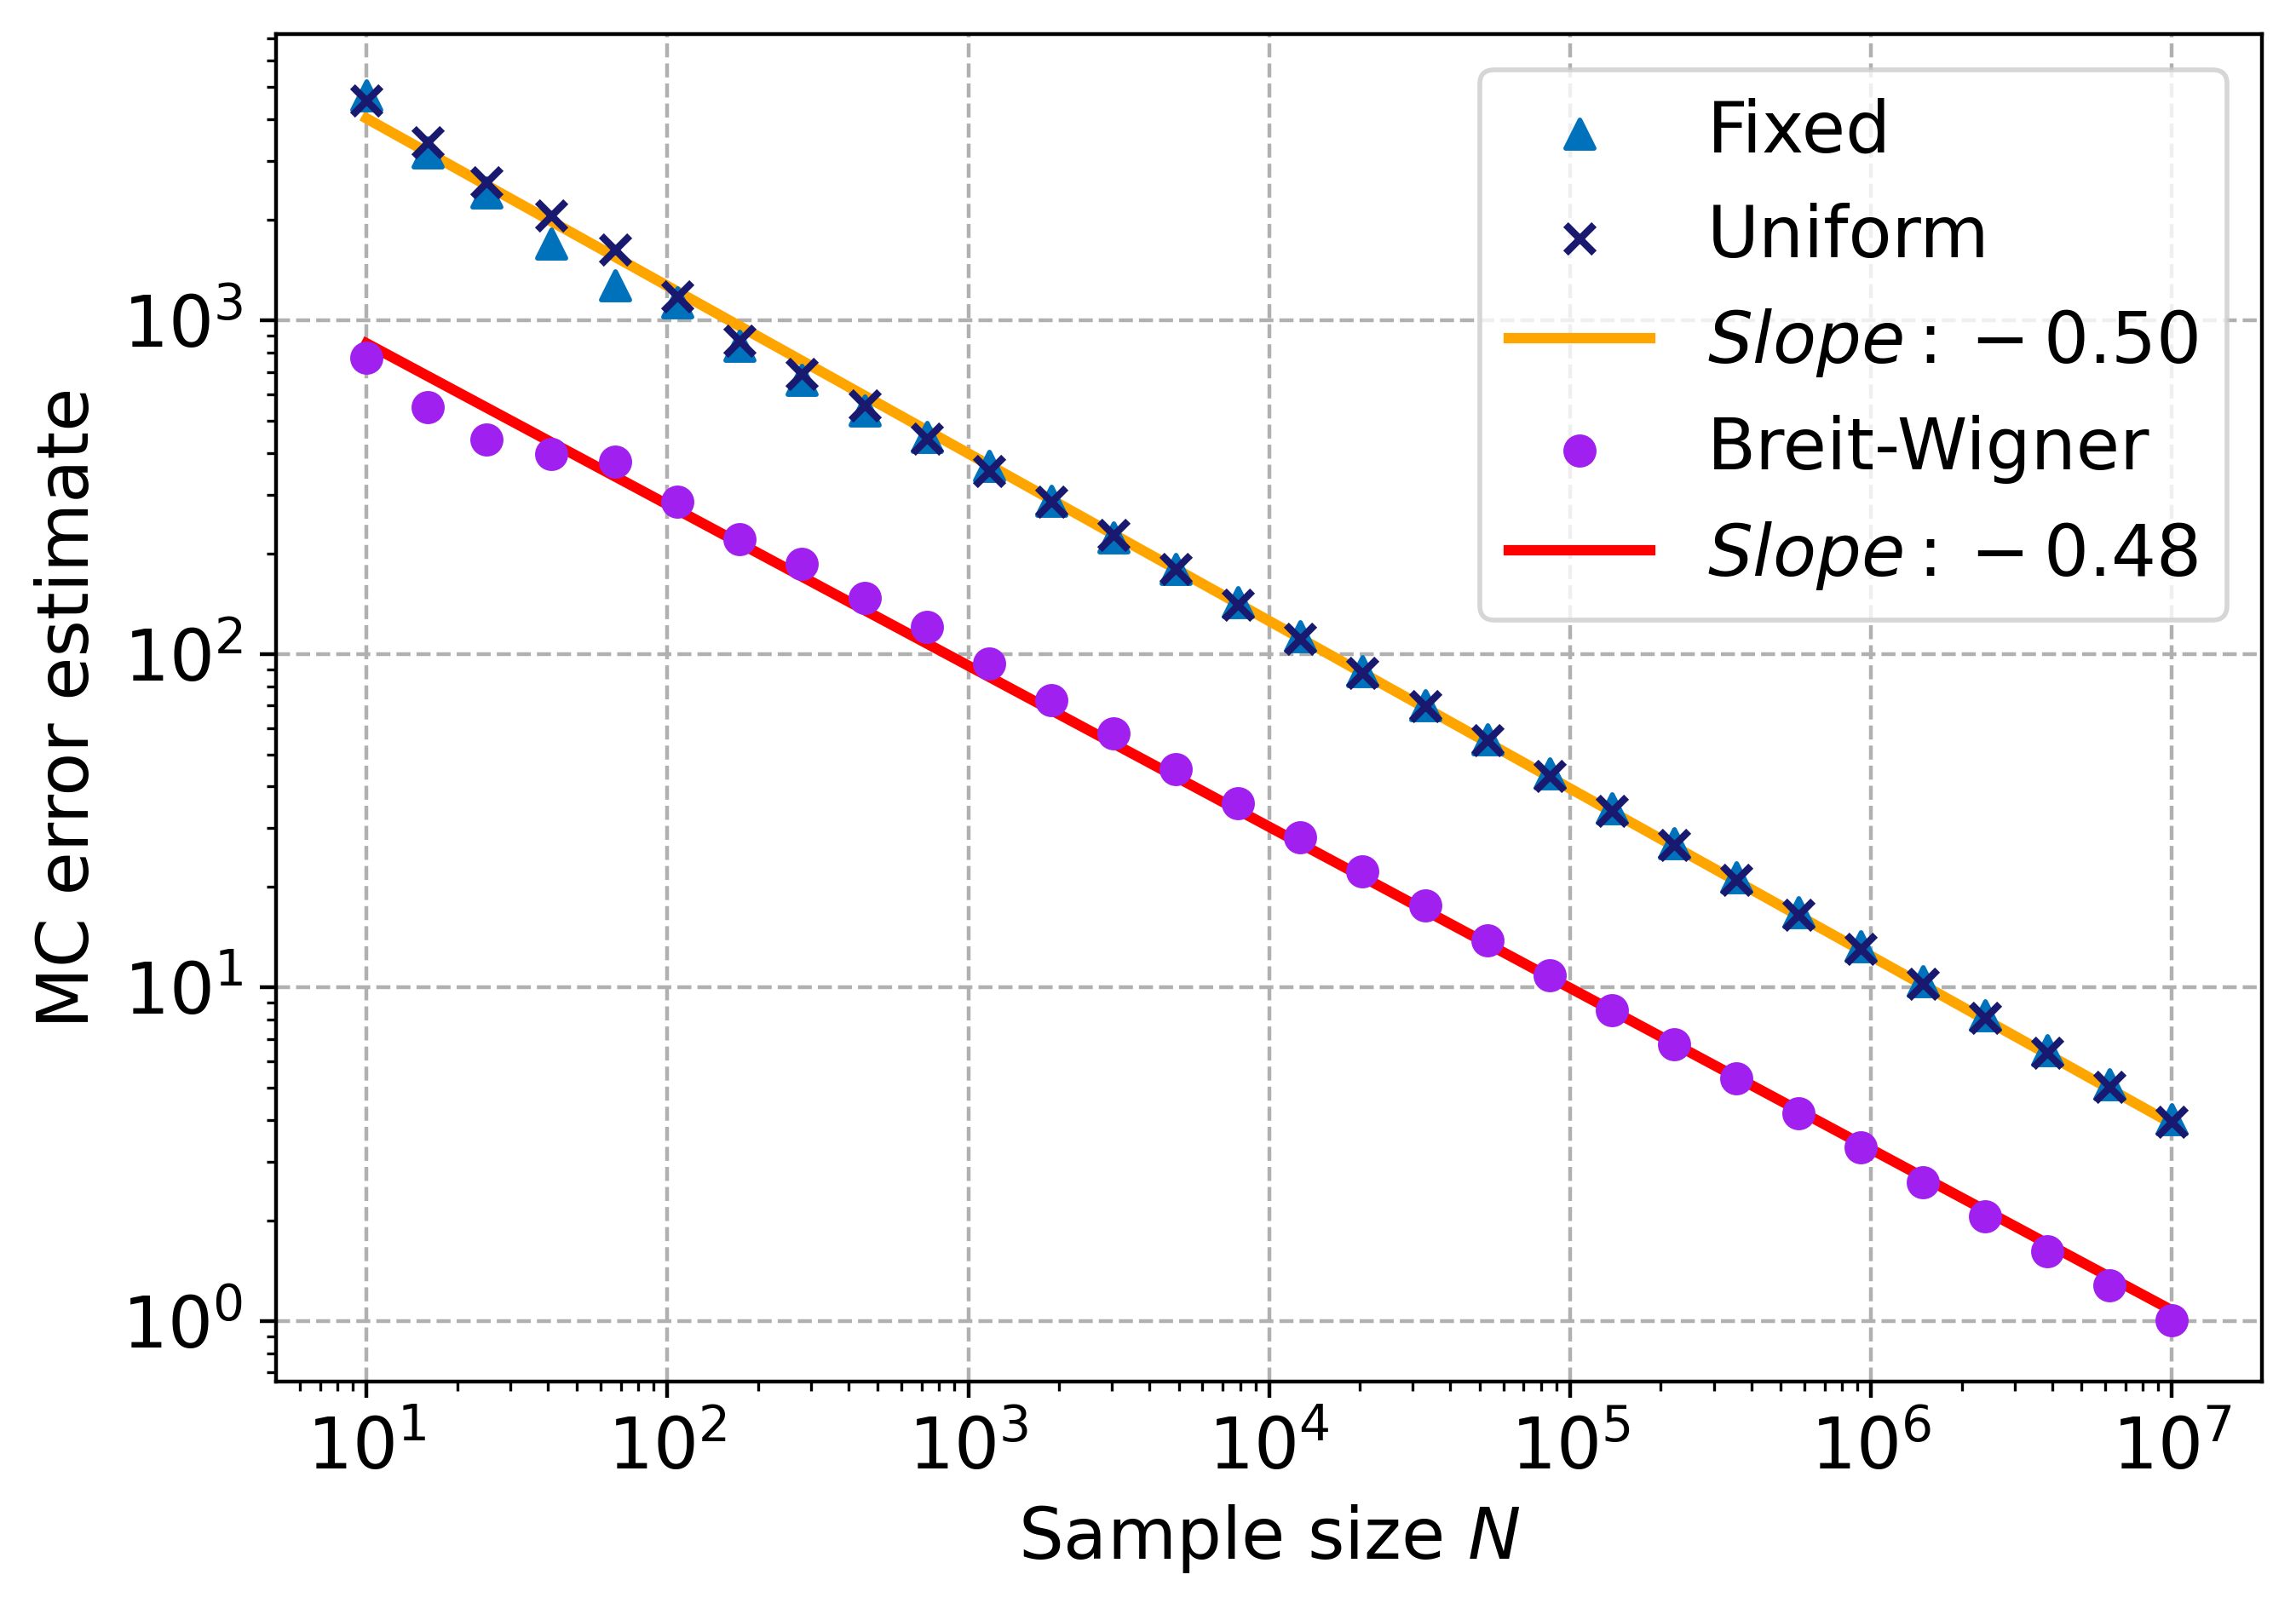
\includegraphics[width=\linewidth]{figures/ex1_all_mc_errors.png}
    \captionof{figure}{Monte Carlo error estimate of the cross-section vs. sample size for the three different cases of $s$ sampling.}
    \label{fig:1-mc-errors}
\end{minipage} \hfill
\begin{minipage}{0.47\linewidth}
    \centering
    \captionsetup{type=figure}
    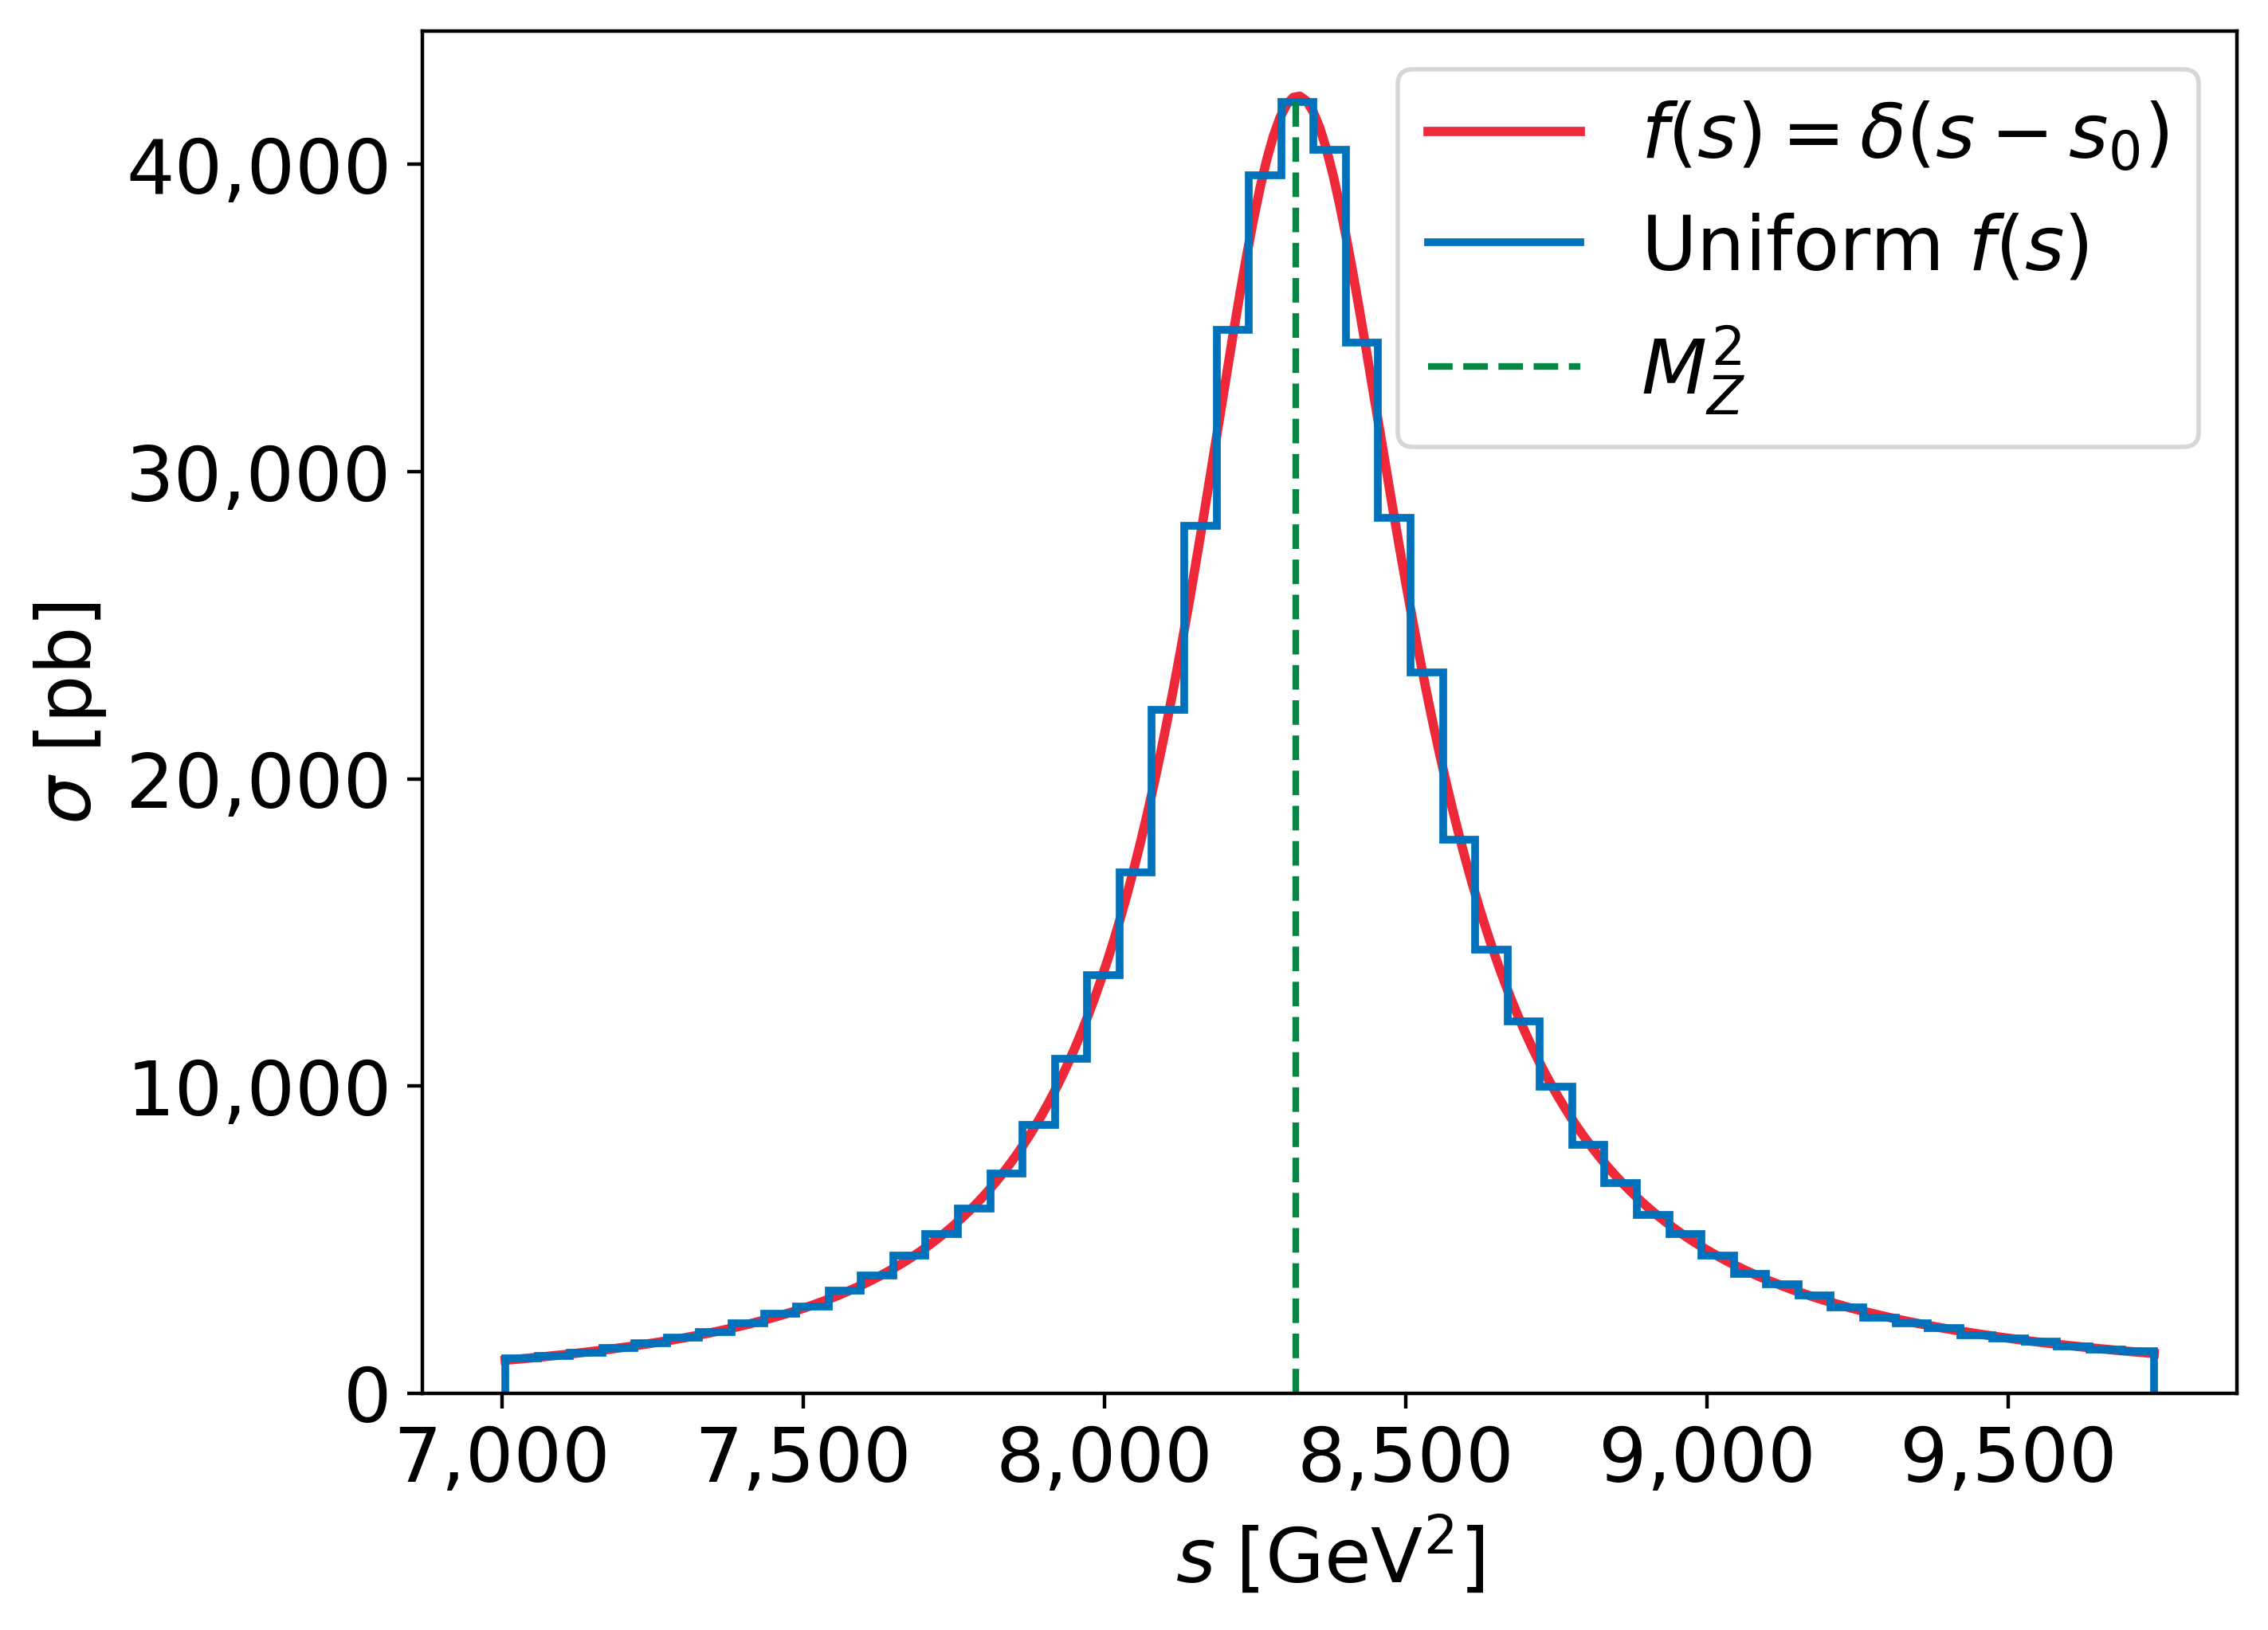
\includegraphics[width=\linewidth]{figures/ex1_part_d_histo.png}
    \captionof{figure}{Cross-section values from binning the flat beam spectrum vs. integration at fixed beam energy.}
    \label{fig:ex1d_histogram}
\end{minipage}

\medskip

The fact that the values of the cross-section are distributed along $s$ in the shape found in \autoref{fig:ex1d_histogram}, is precisely what motivates sampling $s$ according to the Breit-Wigner distribution with the Z boson as the resonance (well, that and the whole theoretical background, of course), equation \eqref{eq:1-breit-wigner}. This distribution has a global maximum at $M_{\mathrm{Z}}^{2}$, decaying to both sides, besides resembling the common factor present in both $\chi_{1}(s)$ and $\chi_{2}(s)$, equation \eqref{eq:1-chi-funcs}. Thus, the Breit-Wigner distribution seems to capture well the importance of different $s$ values to the integral for the cross-section, providing a more reasonable distribution for sampling $s$ rather than a uniform distribution. This is indeed the case, as can be seen from the Monte Carlo error estimates in \autoref{tab:1-cross-sections} and \autoref{fig:1-mc-errors}, where \marginpar{Part g)}\emph{the errors are four times smaller than the uniform case for the same sample size}.

\subsection{Vegas}

The improvement in accuracy of Monte Carlo methods when estimating integrals, as a result of using importance sampling with a distribution that captures enough features of the integrand, has led to develop sophisticated algorithms to determine such distributions. An example of these, is the implementation of Monte Carlo integration in the \texttt{vegas} package for python. This package implements the VEGAS algorithm, consisting on “scanning” over several passes the integration region and making a histogram that approximates the distribution of the integrand. In particular, the package implements two adaptive strategies: importance sampling and adaptive stratified sampling. Thus, an integration problem using the \texttt{vegas.Integrator}\textsuperscript{\texttrademark} is characterized solely by a region of integration and an integrand. After this, a number of evaluations \texttt{neval} (how many times to evaluate the integrand) and a number of iterations \texttt{nint} (number of times to perform \texttt{neval} evaluations of the integrand) yield independent estimations of the integral. A complete discussion of its implementation and use of the package can be found in \url{https://vegas.readthedocs.io/en/latest/tutorial.html}. 

Using 10 iterations with 1,000 Monte Carlo points each, the differential cross-section in equation \eqref{eq:1-diff-sigma} was integrated with \texttt{vegas}, obtaining the results shown in \autoref{tab:1-vegas-summary}. Here, the first two iterations are not to be taken into account, shown by the relatively high values of $Q$ (the $p$-value of the $\chi^{2}$) as compared with the rest of the subsequent iterations. This is because during these iterations vegas has not yet been able to fully optimize the sampling for the integrand. However, for every iteration after the second, the error decreases consistently, reaching a weighted average result of 9,930 pb with an error estimate of 14 pb, only 1pb of difference from the exact value of 9,929 pb.

\begin{table}[ht!]
    \centering
    \renewcommand{\arraystretch}{1.2}
    \begin{tabular}{rcccc}
    \hline Iteration & Integral & Weighted average & $\chi^{2} /$ d.o.f. & $Q$ \\ \hline
    1 & 9,720(17) & 9,720(17) & 0.00 & 1.00 \\
    2 & 10,030(10) & 9,948(87) & 2.54 & 0.11 \\
    3 & 9,653(79) & 9,787(59) & 4.42 & 0.01 \\
    4 & 9,952(70) & 9,855(45) & 4.05 & 0.01 \\
    5 & 9,933(54) & 9,887(35) & 3.34 & 0.01 \\
    6 & 9,933(52) & 9,901(29) & 2.79 & 0.02 \\
    7 & 9,878(42) & 9,894(24) & 2.35 & 0.03 \\
    8 & 9,899(38) & 9,895(20) & 2.02 & 0.05 \\
    9 & 9950(33) & 9,910(17) & 2.01 & 0.04 \\
    10 & 9,977(26) & 9,930(14) & 2.29 & 0.01 \\ \hline
    \end{tabular}
    \caption{Summary of the vegas integration for 10 iterations of 1,000 Monte Carlo points each. The “Integral” and “Weighted average” columns correspond to estimations for the cross-section in picobarns. $Q$ represents the $p$-value of the $\chi^{2}$.}
    \label{tab:1-vegas-summary}
\end{table}

The remarkably good estimation for the cross-section with relatively few evaluations is made possible due to the fact that \texttt{vegas} has been able to “flatten” the integral, i.e., find a transformation of the integration variables such that their sampling captures better the integrand. This can be seen in \autoref{fig:ex1e_one_grid}, which shows the optimal integration grid found by vegas for the variables $s$ and $\cos{\theta}$ (since there is no dependence on $\phi$). The other two integration grids, for the pairs $(s, \phi)$ and $(\cos{\theta}, \phi)$, are shown in \autoref{sec:app-int-grids}. Although the accumulation of $s$ values close to $M_{\text{Z}}^{2}$ was to be expected, \marginpar{Part e)} \emph{smaller binning for values of $\cos{\theta}$ close to +1 and -1 come as a surprise}. Indeed, this is made clear by plotting the integrand, as shown in \autoref{fig:ex1e-integrand-plot}, where peaks towards these values can be seen, and the peak at +1 is larger than that at $-1$.

\begin{figure}[ht!]
    \centering
    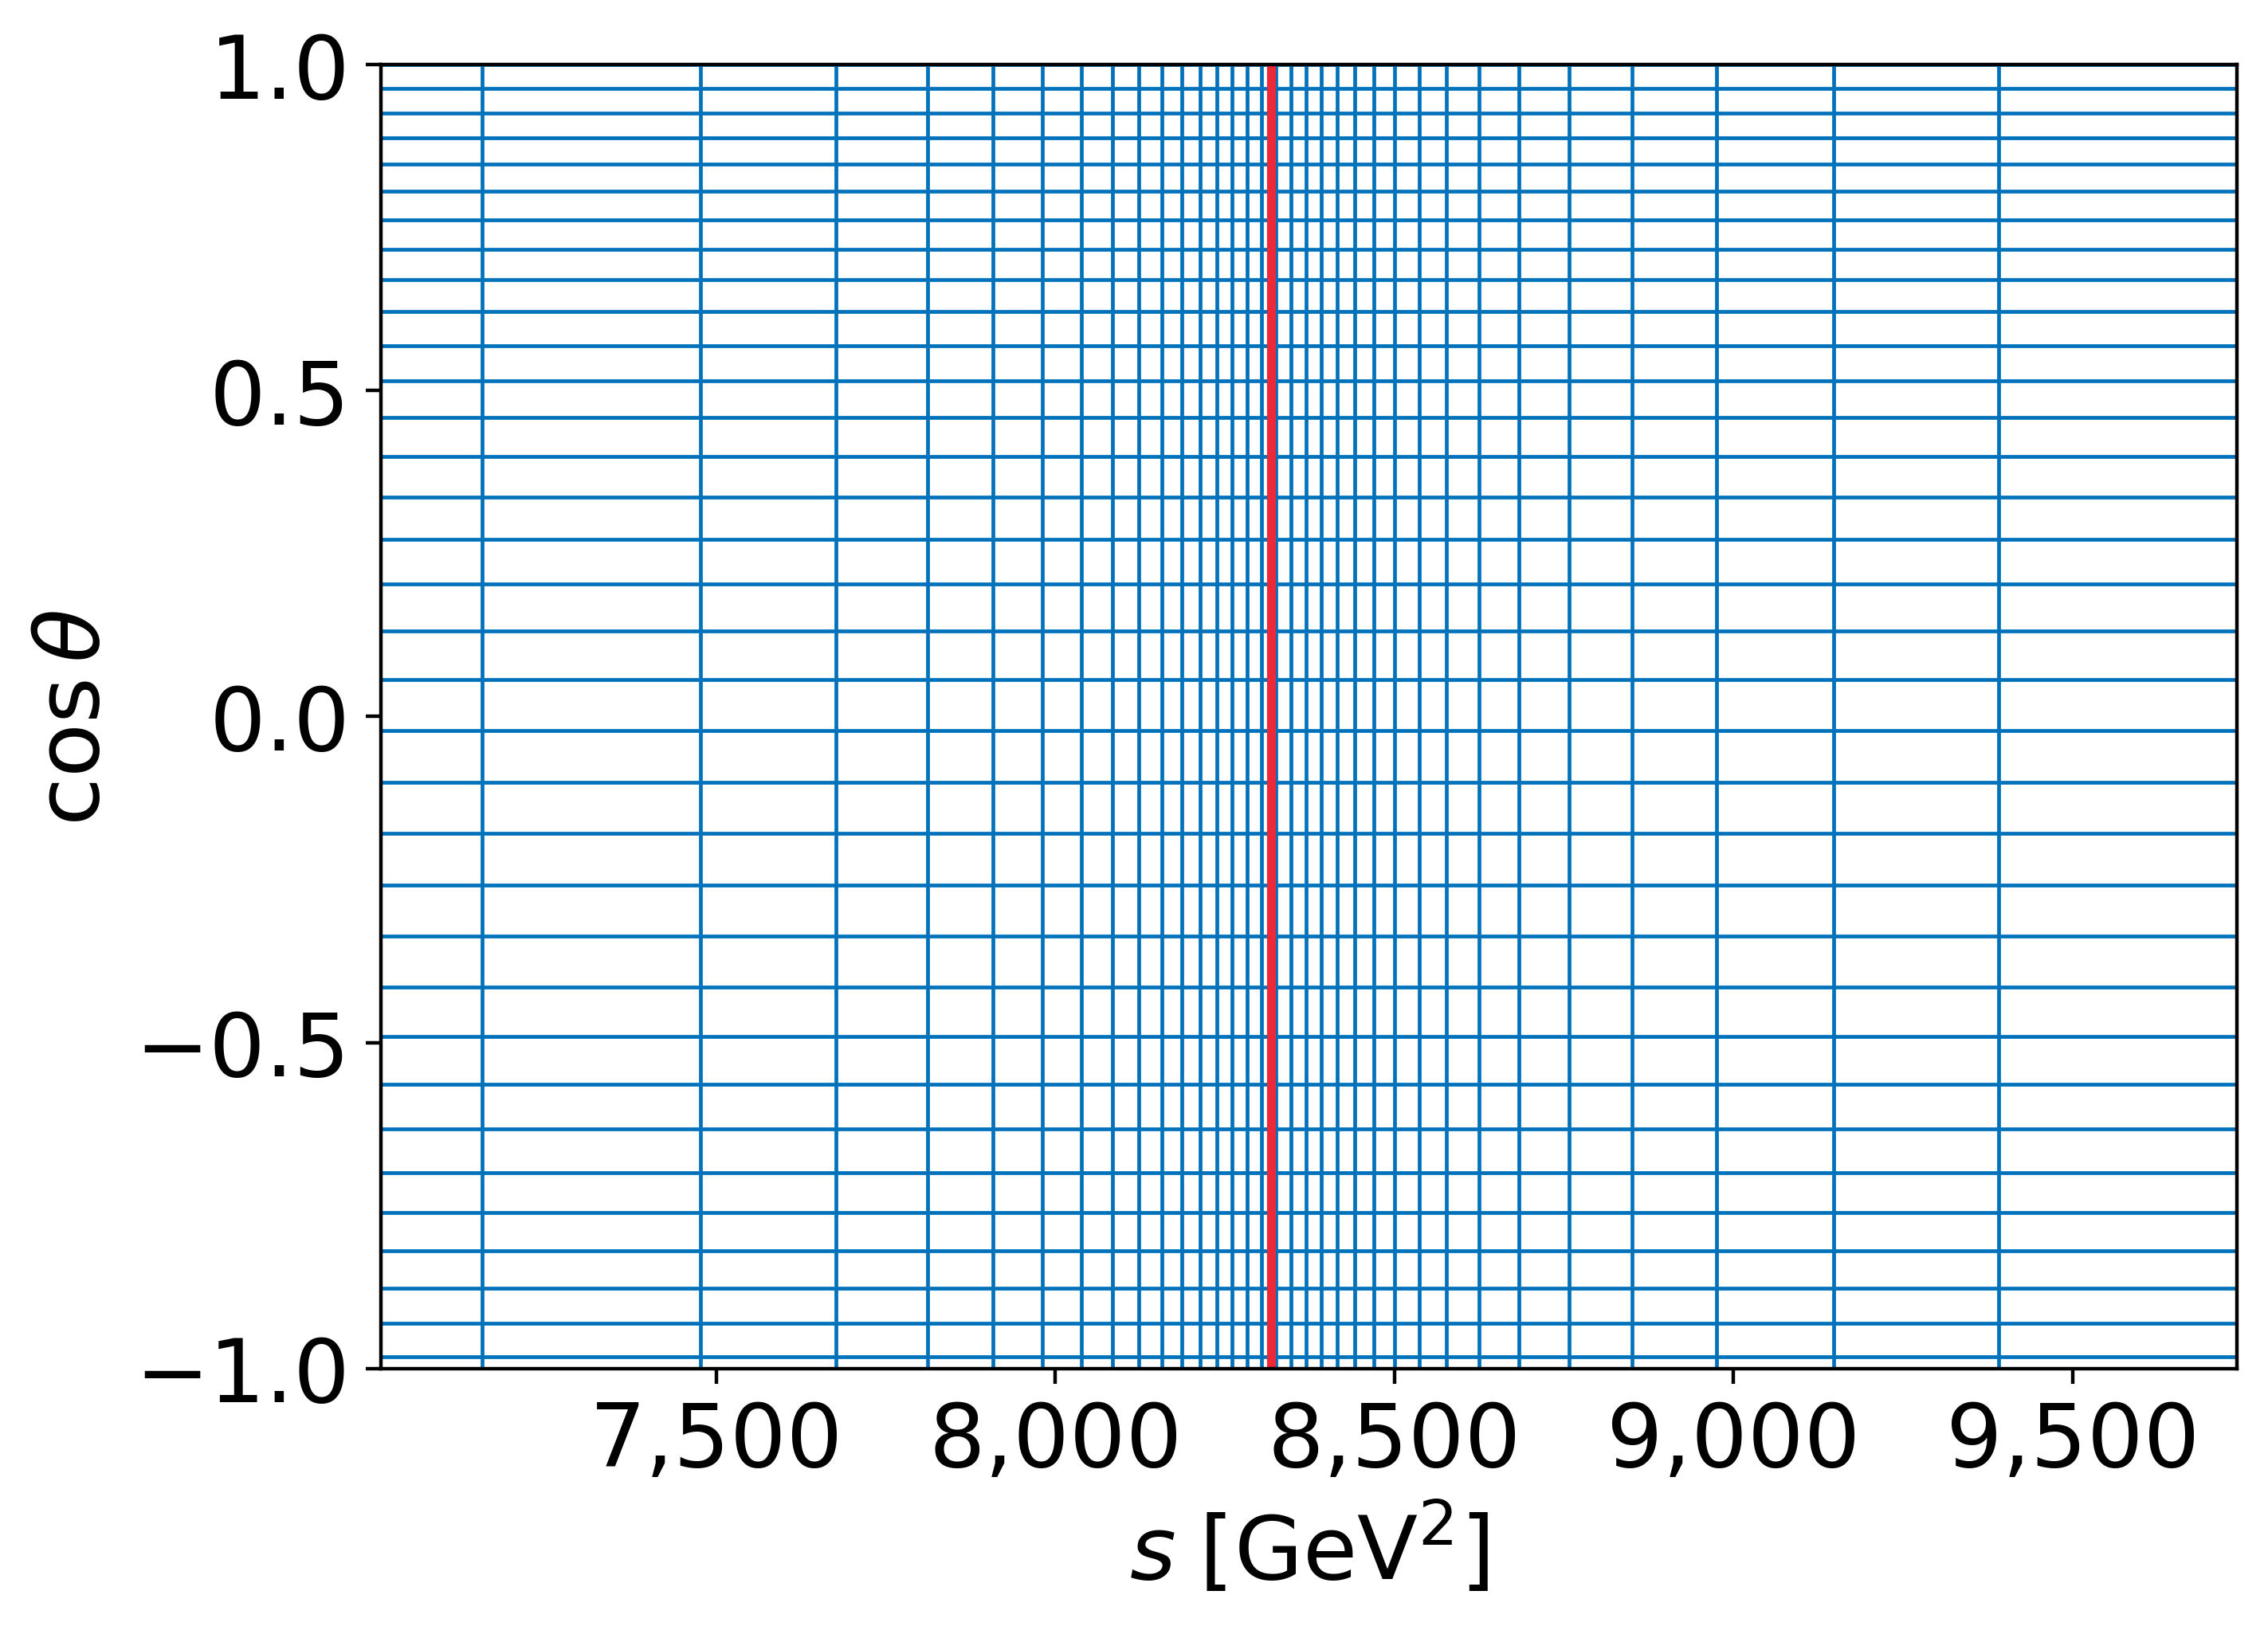
\includegraphics[width=0.6\linewidth]{figures/integration_grid_0.png}
    \caption{Binning of the integration grid found by \texttt{vegas} after 10 iterations of 1,000 evaluations each.}
    \label{fig:ex1e_one_grid}
\end{figure}

\begin{figure}
    \centering
    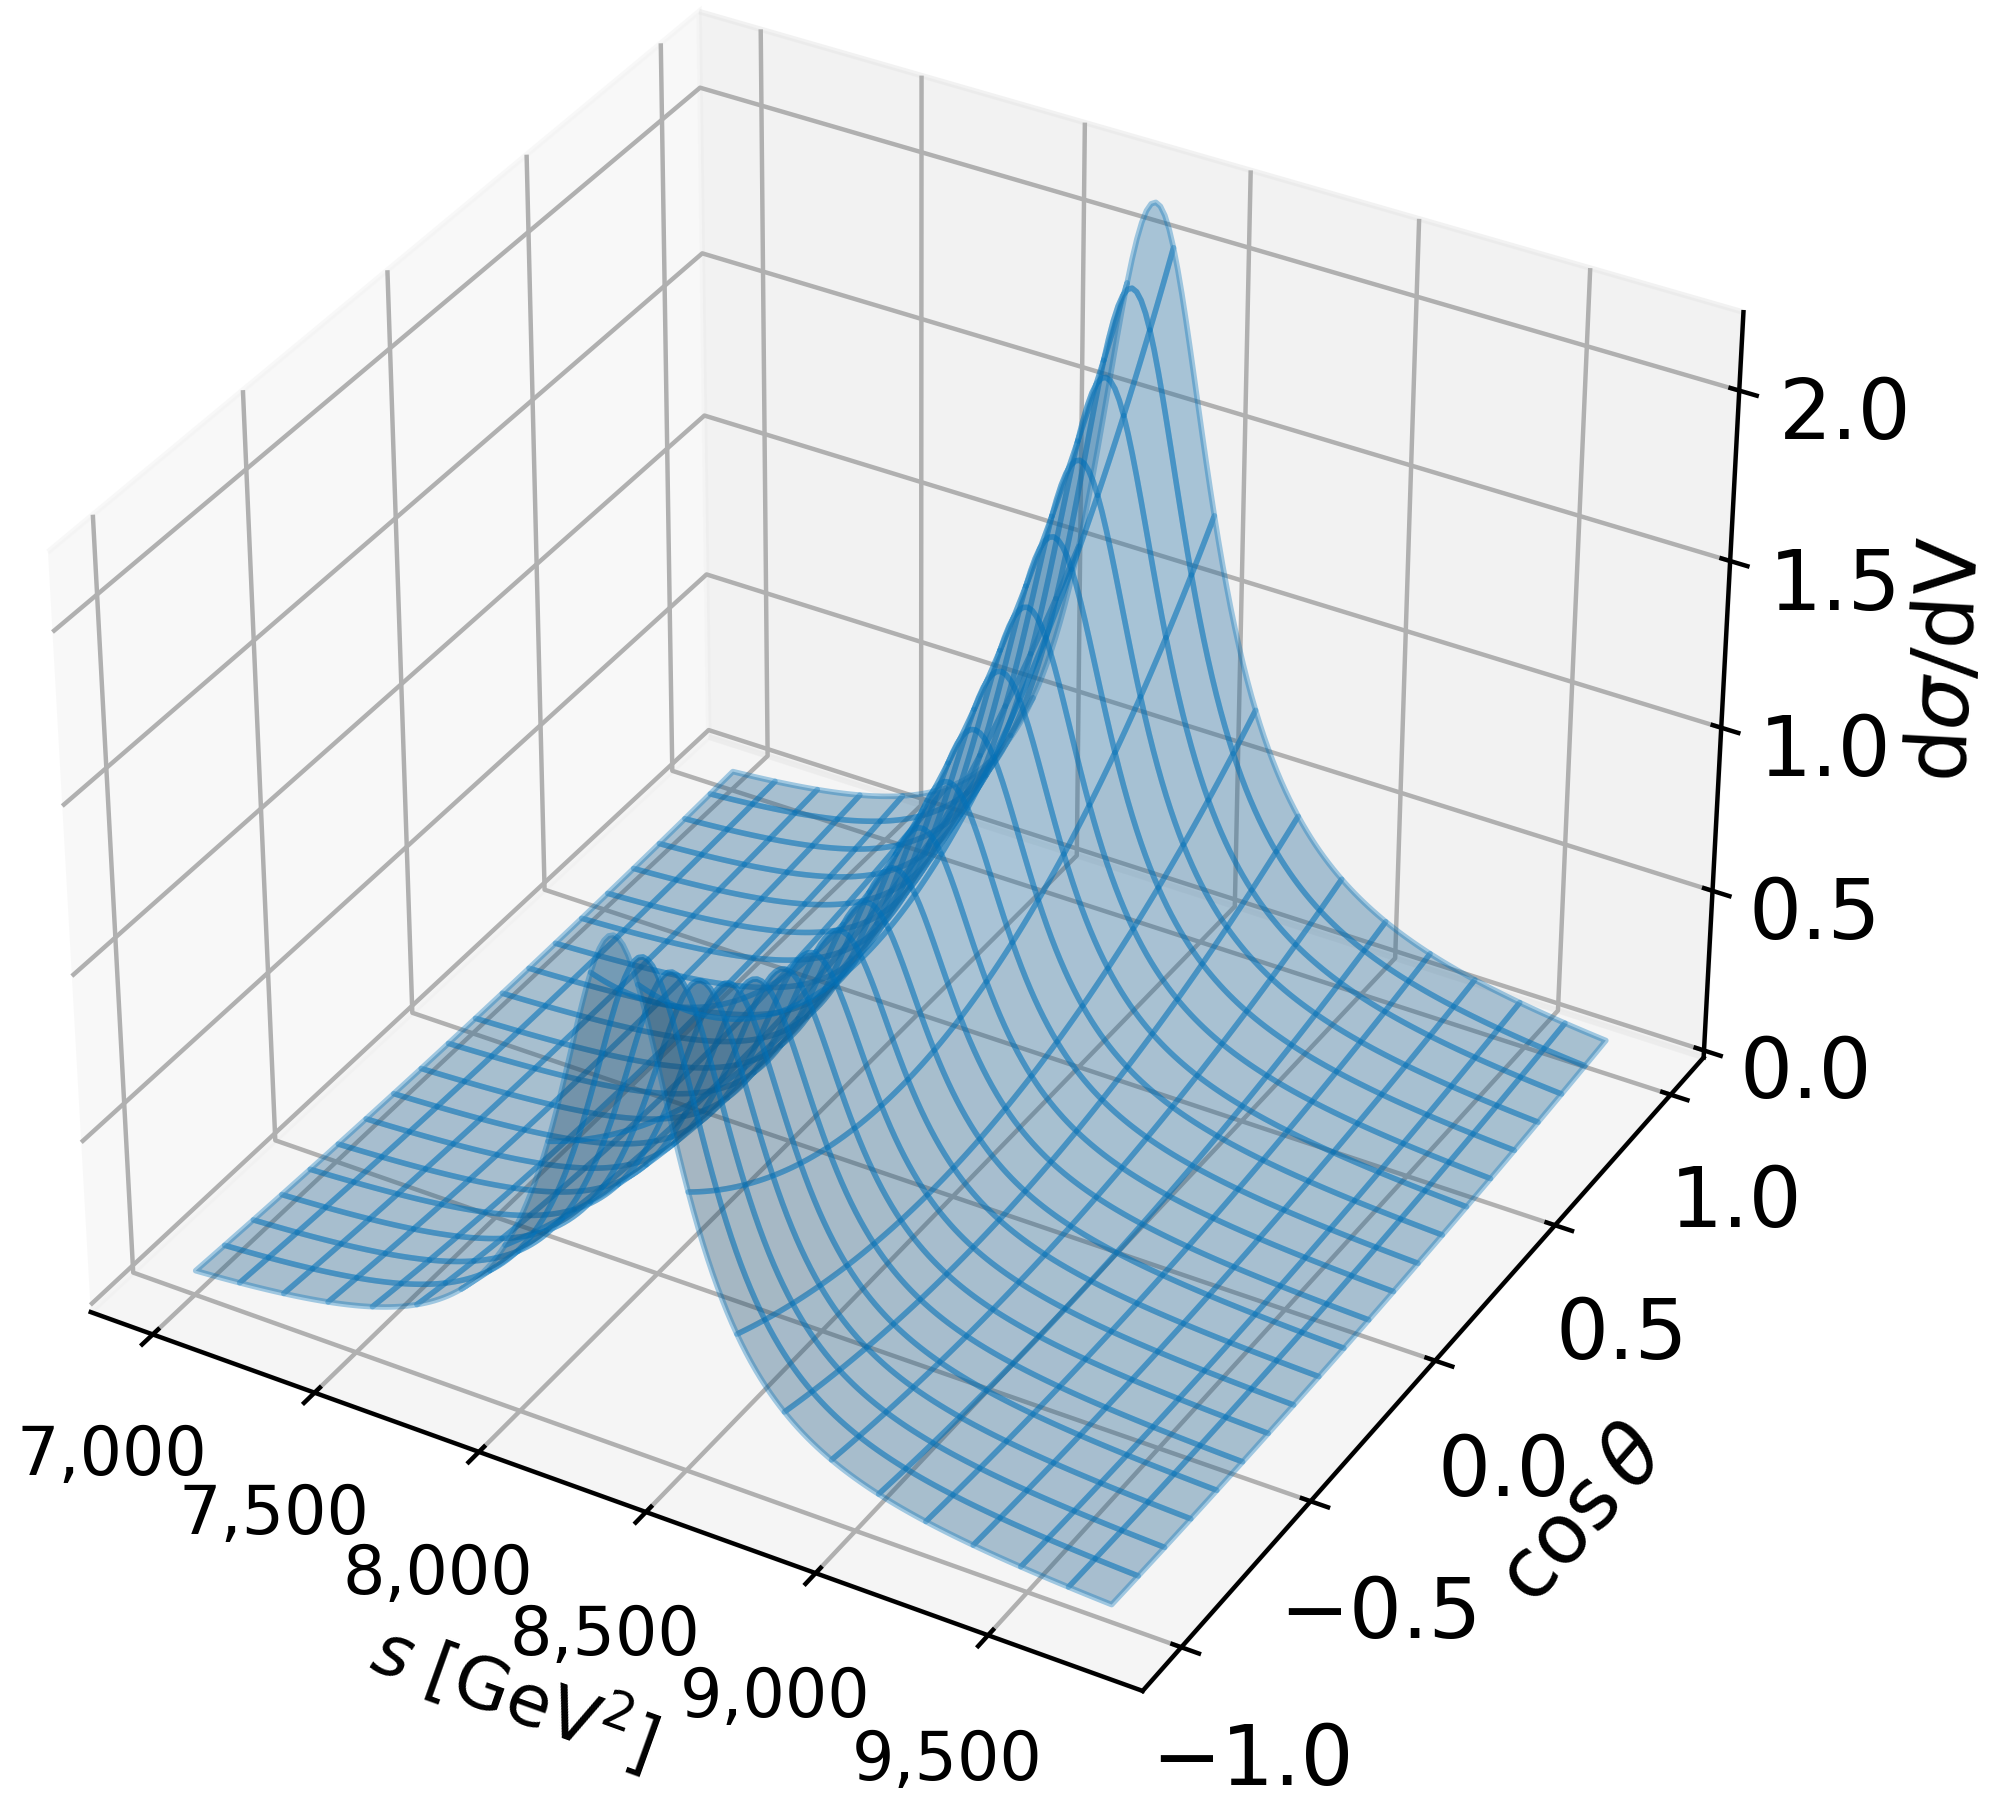
\includegraphics[width=0.6\linewidth]{figures/integrand_plot.png}
    \caption{Differential cross-section per volume. Here $\mathrm{d}V = \mathrm{d}s \, \mathrm{d}(\cos{\theta}) \mathrm{d}\phi$.}
    \label{fig:ex1e-integrand-plot}
\end{figure}

% \begin{minipage}{0.47\linewidth}
%     \centering
%     \captionsetup{type=figure}
%     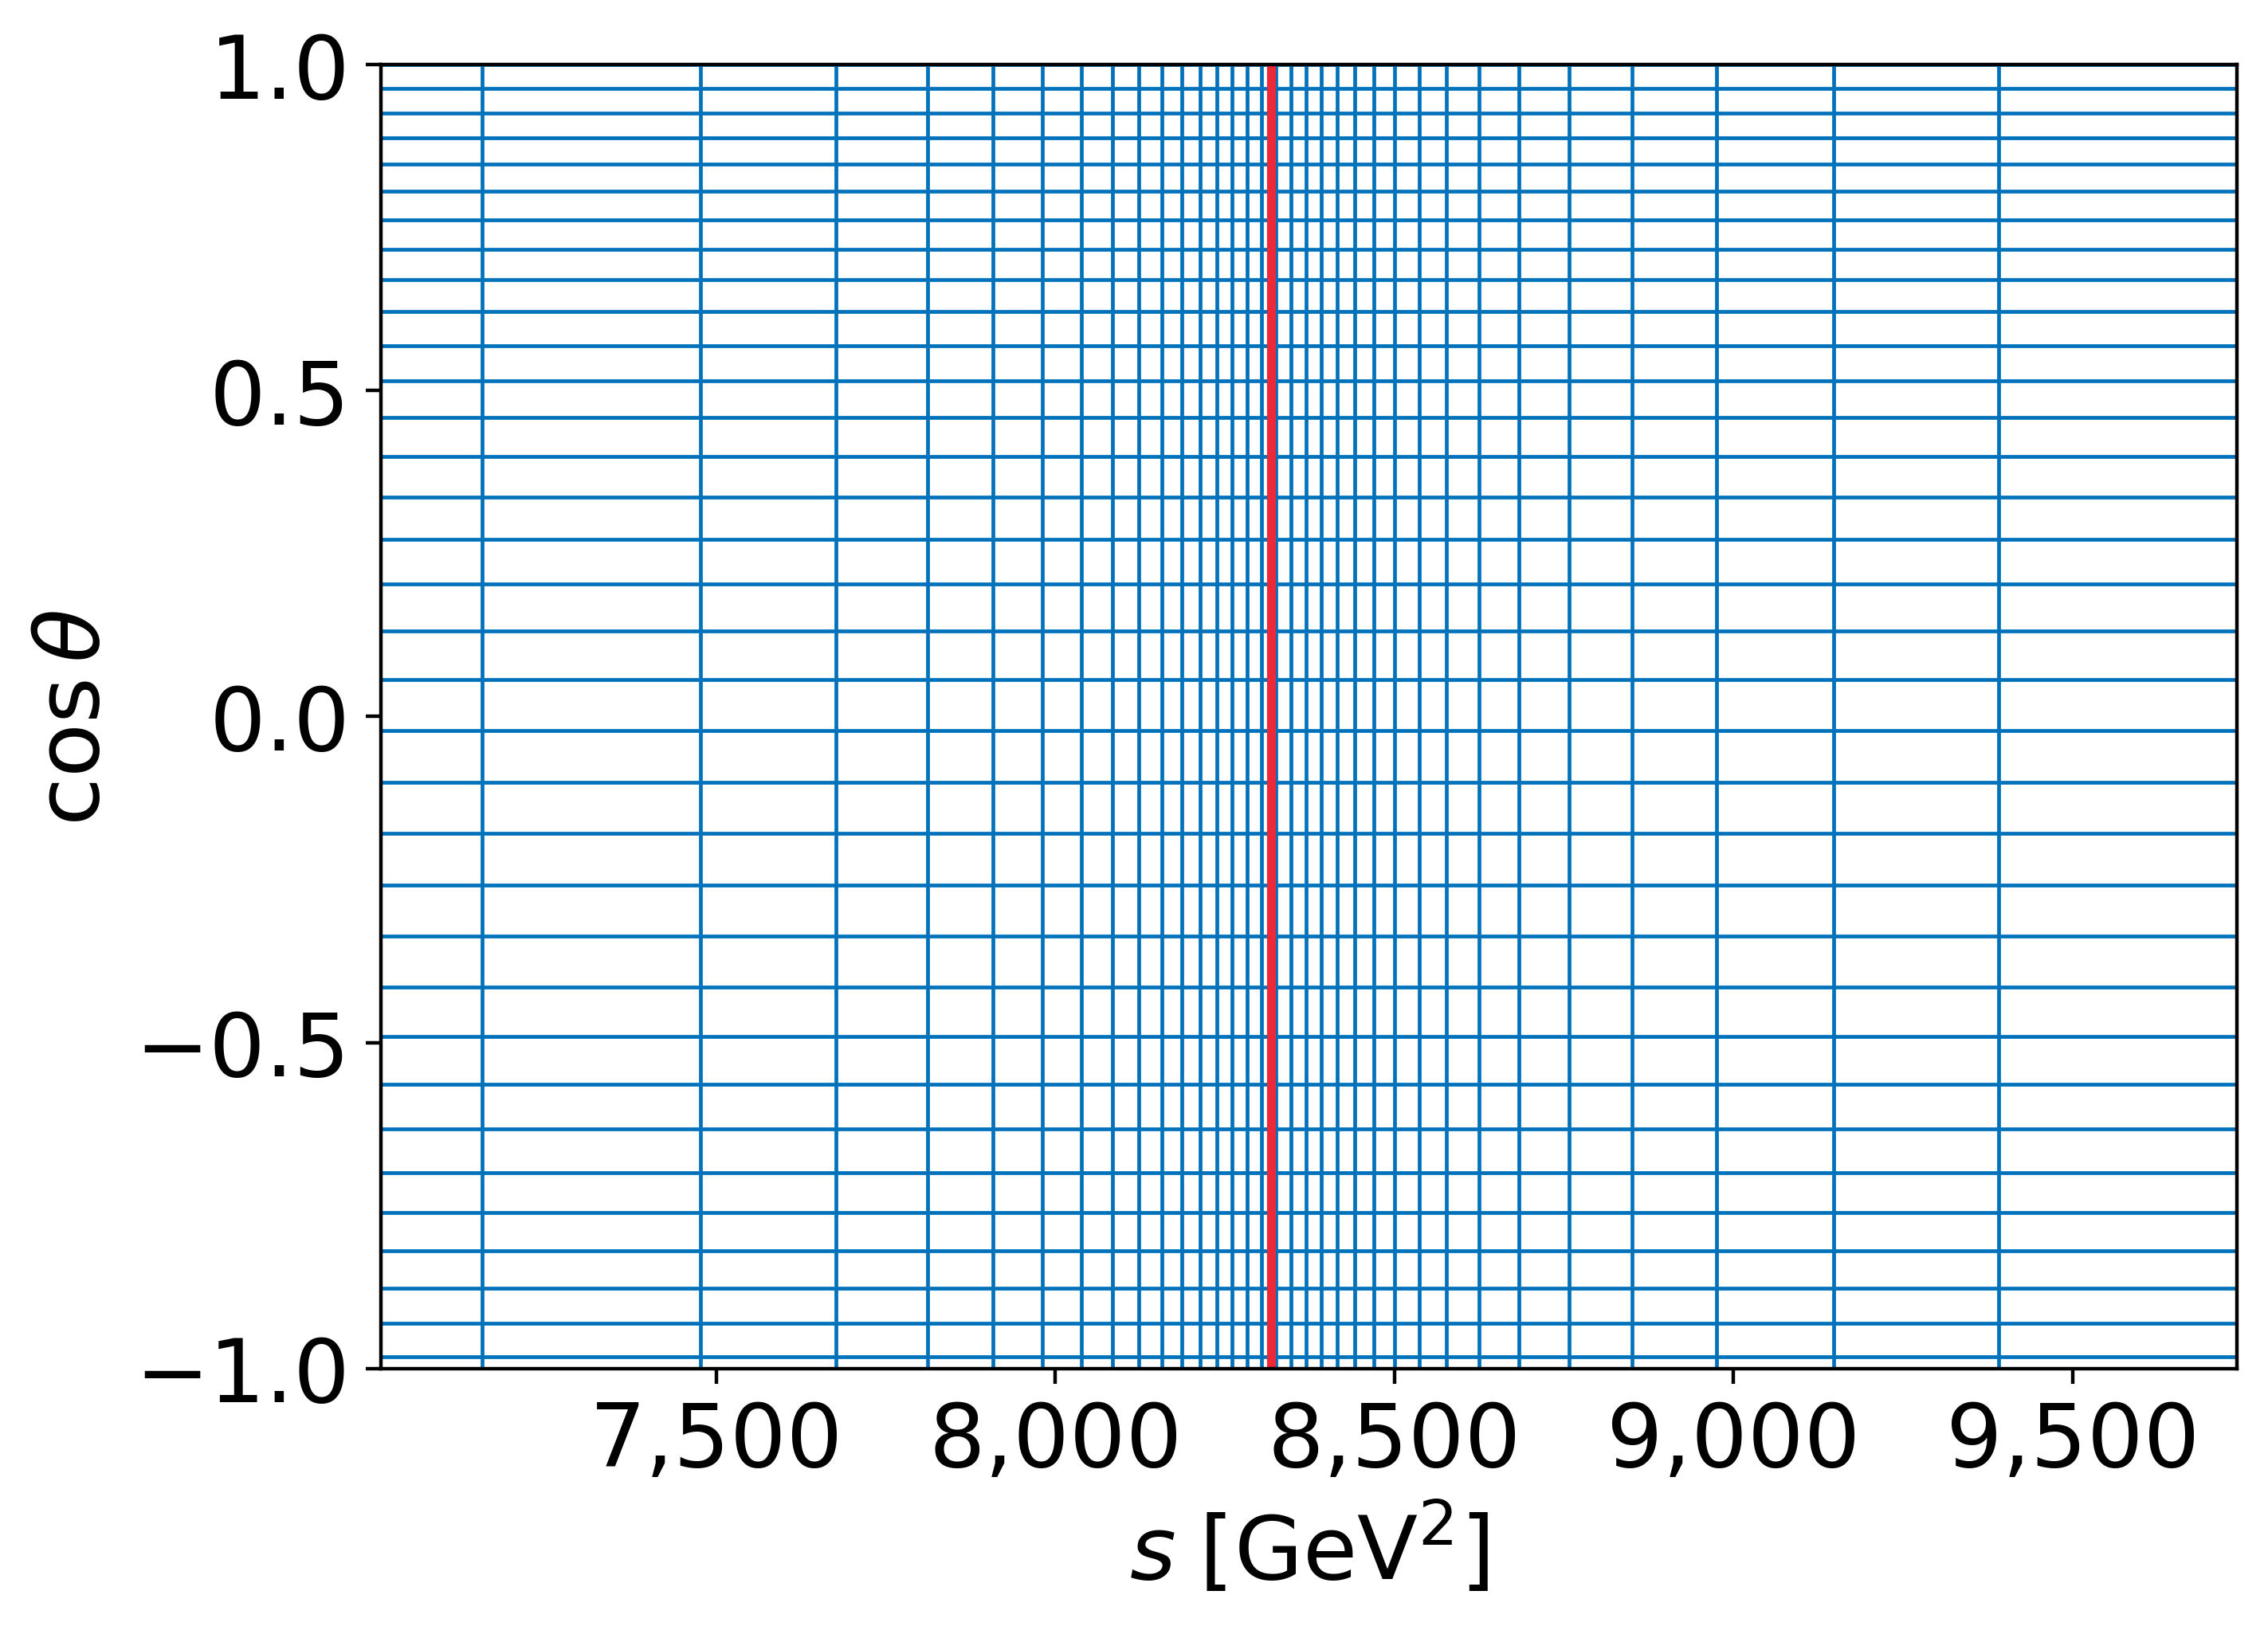
\includegraphics[width=\linewidth]{figures/integration_grid_0.png}
%     \caption{Binning of the integration grid found by \texttt{vegas} after 10 iterations of 1,000 evaluations each.}
%     \label{fig:ex1e_one_grid}
% \end{minipage} \hfill
% \begin{minipage}{0.47\linewidth}
%     \centering
%     \captionsetup{type=figure}
%     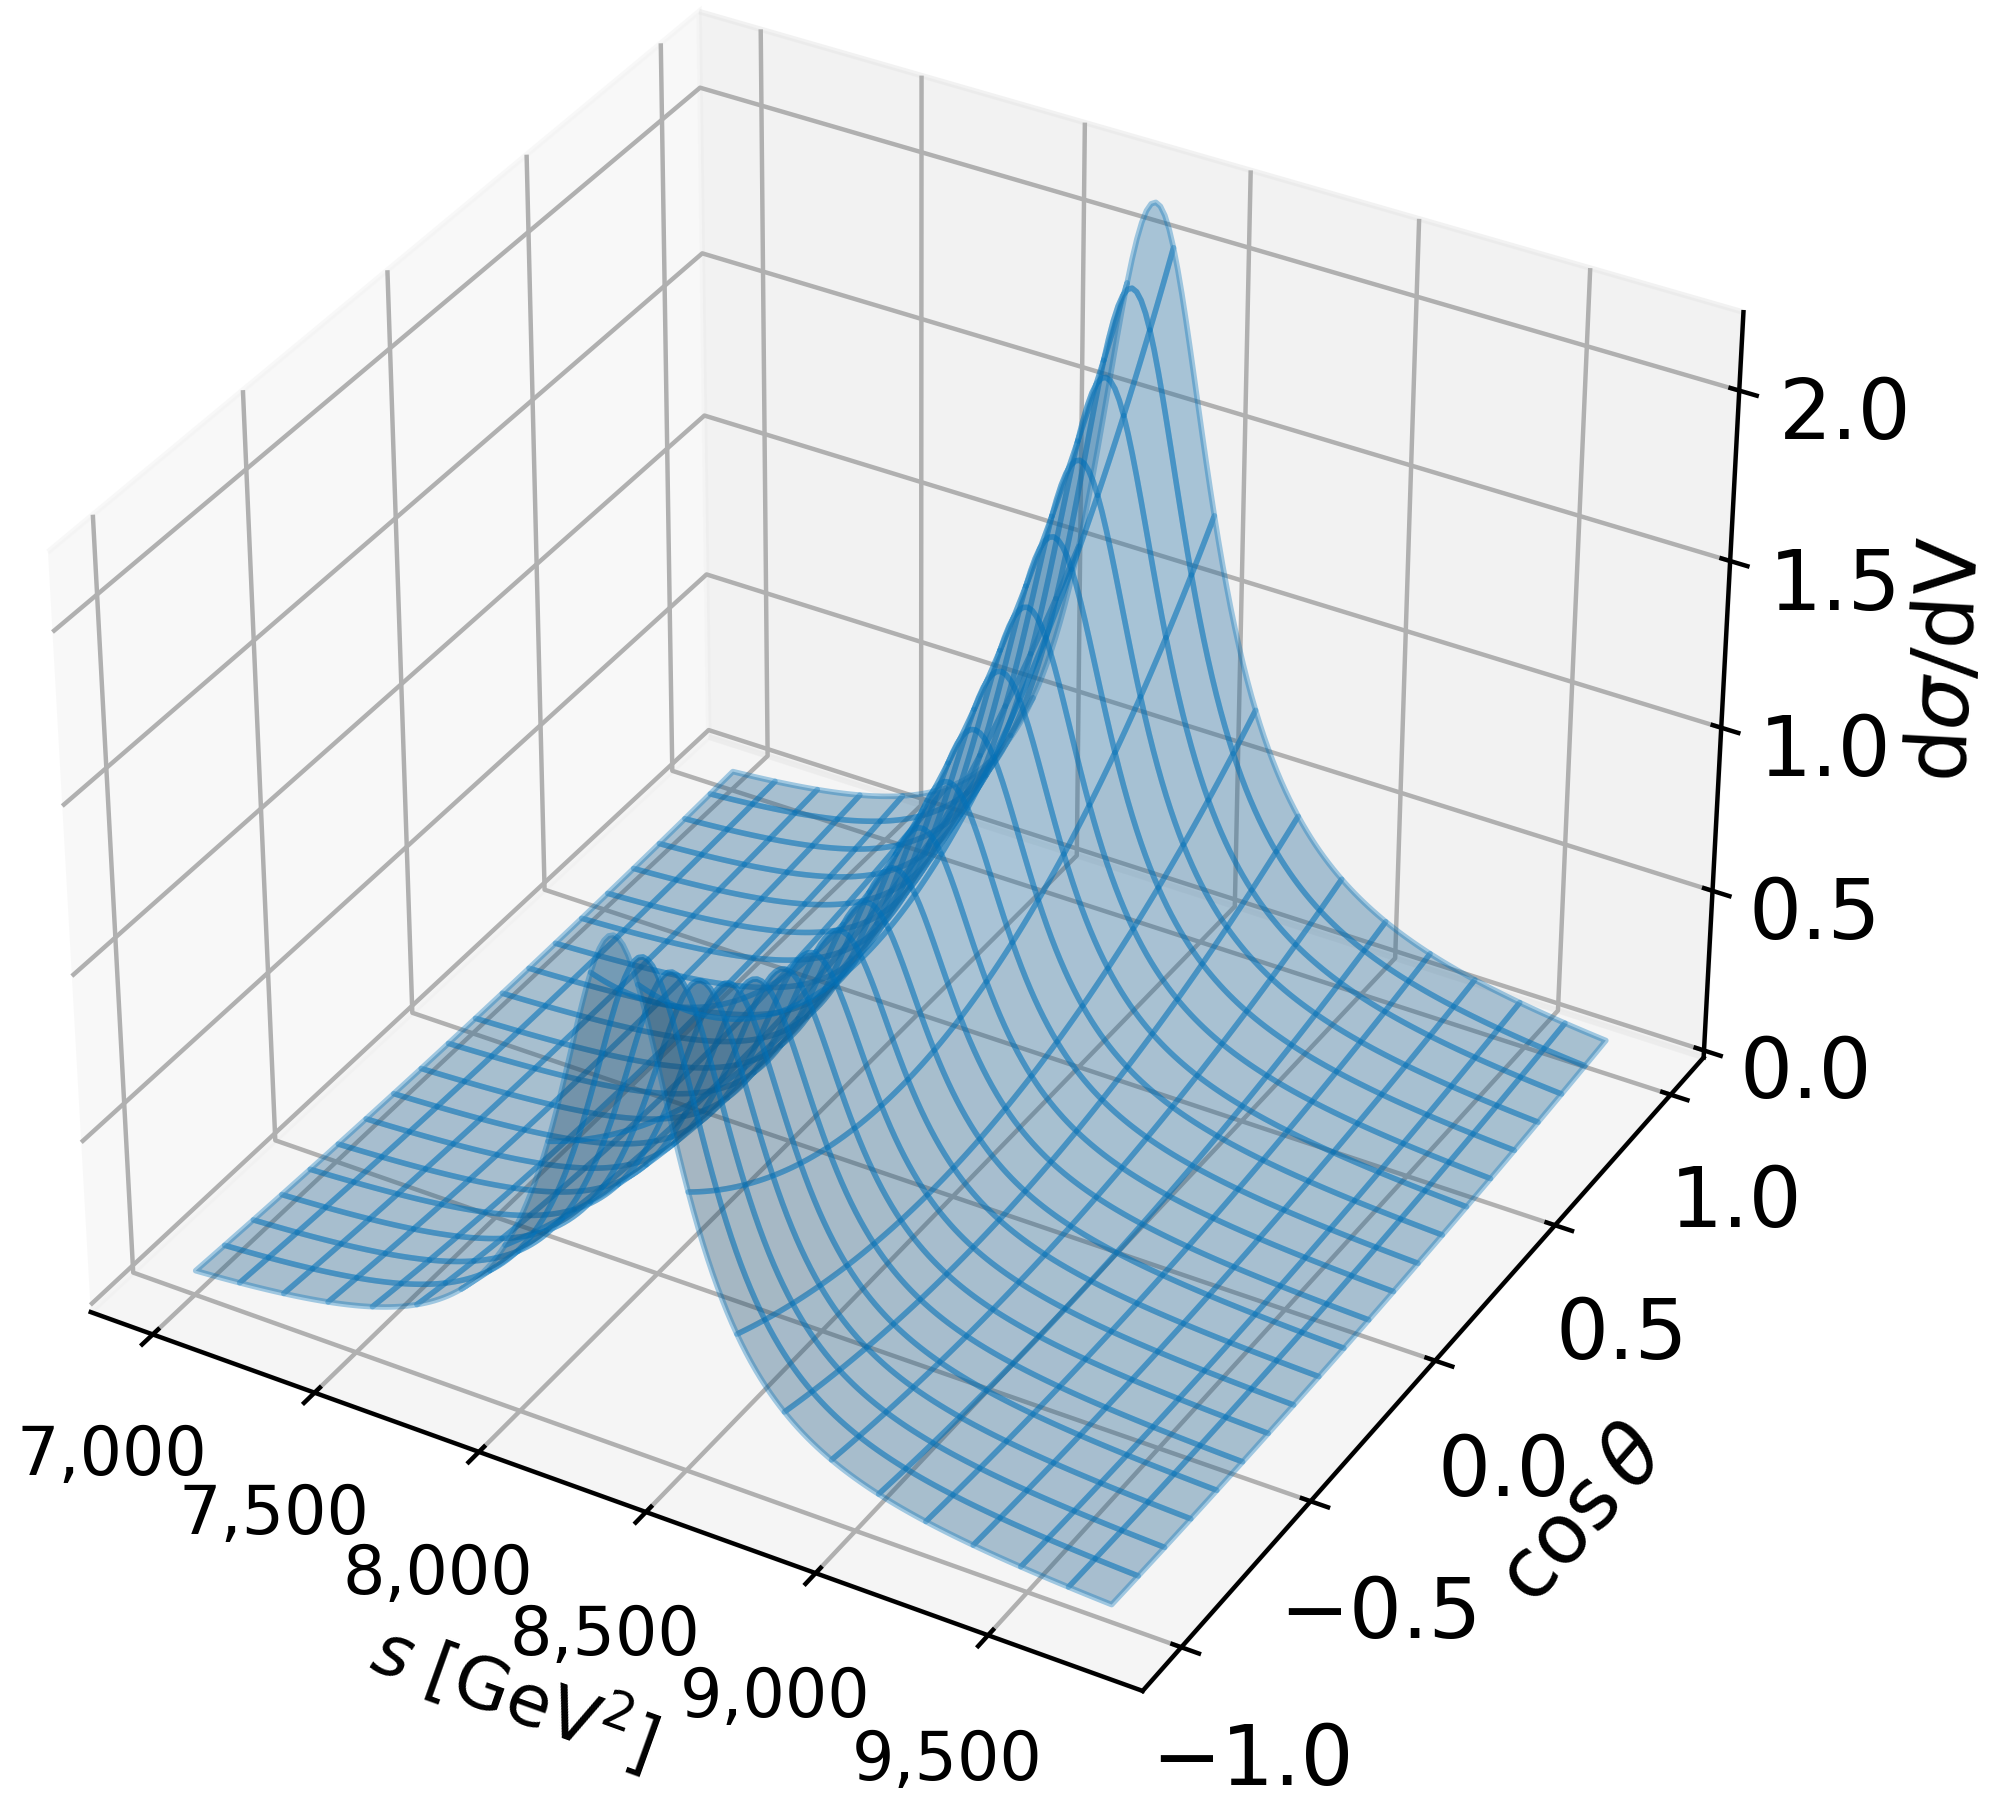
\includegraphics[width=\linewidth]{figures/integrand_plot.png}
%     \captionof{figure}{Differential cross-section per volume. Here $\mathrm{d}V = \mathrm{d}s \, \mathrm{d}(\cos{\theta}) \mathrm{d}\phi$.}
%     \label{fig:ex1e-integrand-plot}
% \end{minipage}


\section{Simulating the bremsstrahlung cascade at all-order QCD}

In the second part of this project, the Monte Carlo integrator from the first part is supplemented with a parton shower, in order to add the effects of additional QCD bremsstrahlung produced by the final-state quark-antiquark pair. After a brief comment on parton showers and the kinematic limit in which it is possible to simulate this cascade at all orders in QCD, the use of the Monte Carlo integrator together with the Parton shower class provided is explained, discussing the change in final-state particles at the end. Finally, jets and jet clustering algorithms are introduced, together with histograms for the differential jet rates produced by the simulation, using as a baseline data produced with \textsc{Sherpa}.

\subsection{Parton Shower}

In the previous section, the leading-order squared matrix element, equation \eqref{eq:1-sqr-mat-element}, is quadratic on the QED coupling $\alpha$. The term “leading-order” implying, in this context, that we are dealing with the smallest possible power in the coupling, thereby neglecting further terms proportional to, e.g. $\alpha^{4}$. This coupling is not constant, however, and its value varies with the energy scale. Fortunately, the variation of the QED coupling at the energy scales relevant for the process here studied, is small: at low energy scales one has $\alpha \approx 1/137$, reaching $\alpha \approx 1 / 127$ at the scale of the Z boson.

Once the quark-antiquark pair is emitted, these accelerated color-charged particles can radiate gluons (\textit{bremsstrahlung}), which in turn can decay emitting more particles, giving rise to a “cascade”. 
\begin{wrapfigure}{r}{0.5\textwidth}
    \centering
    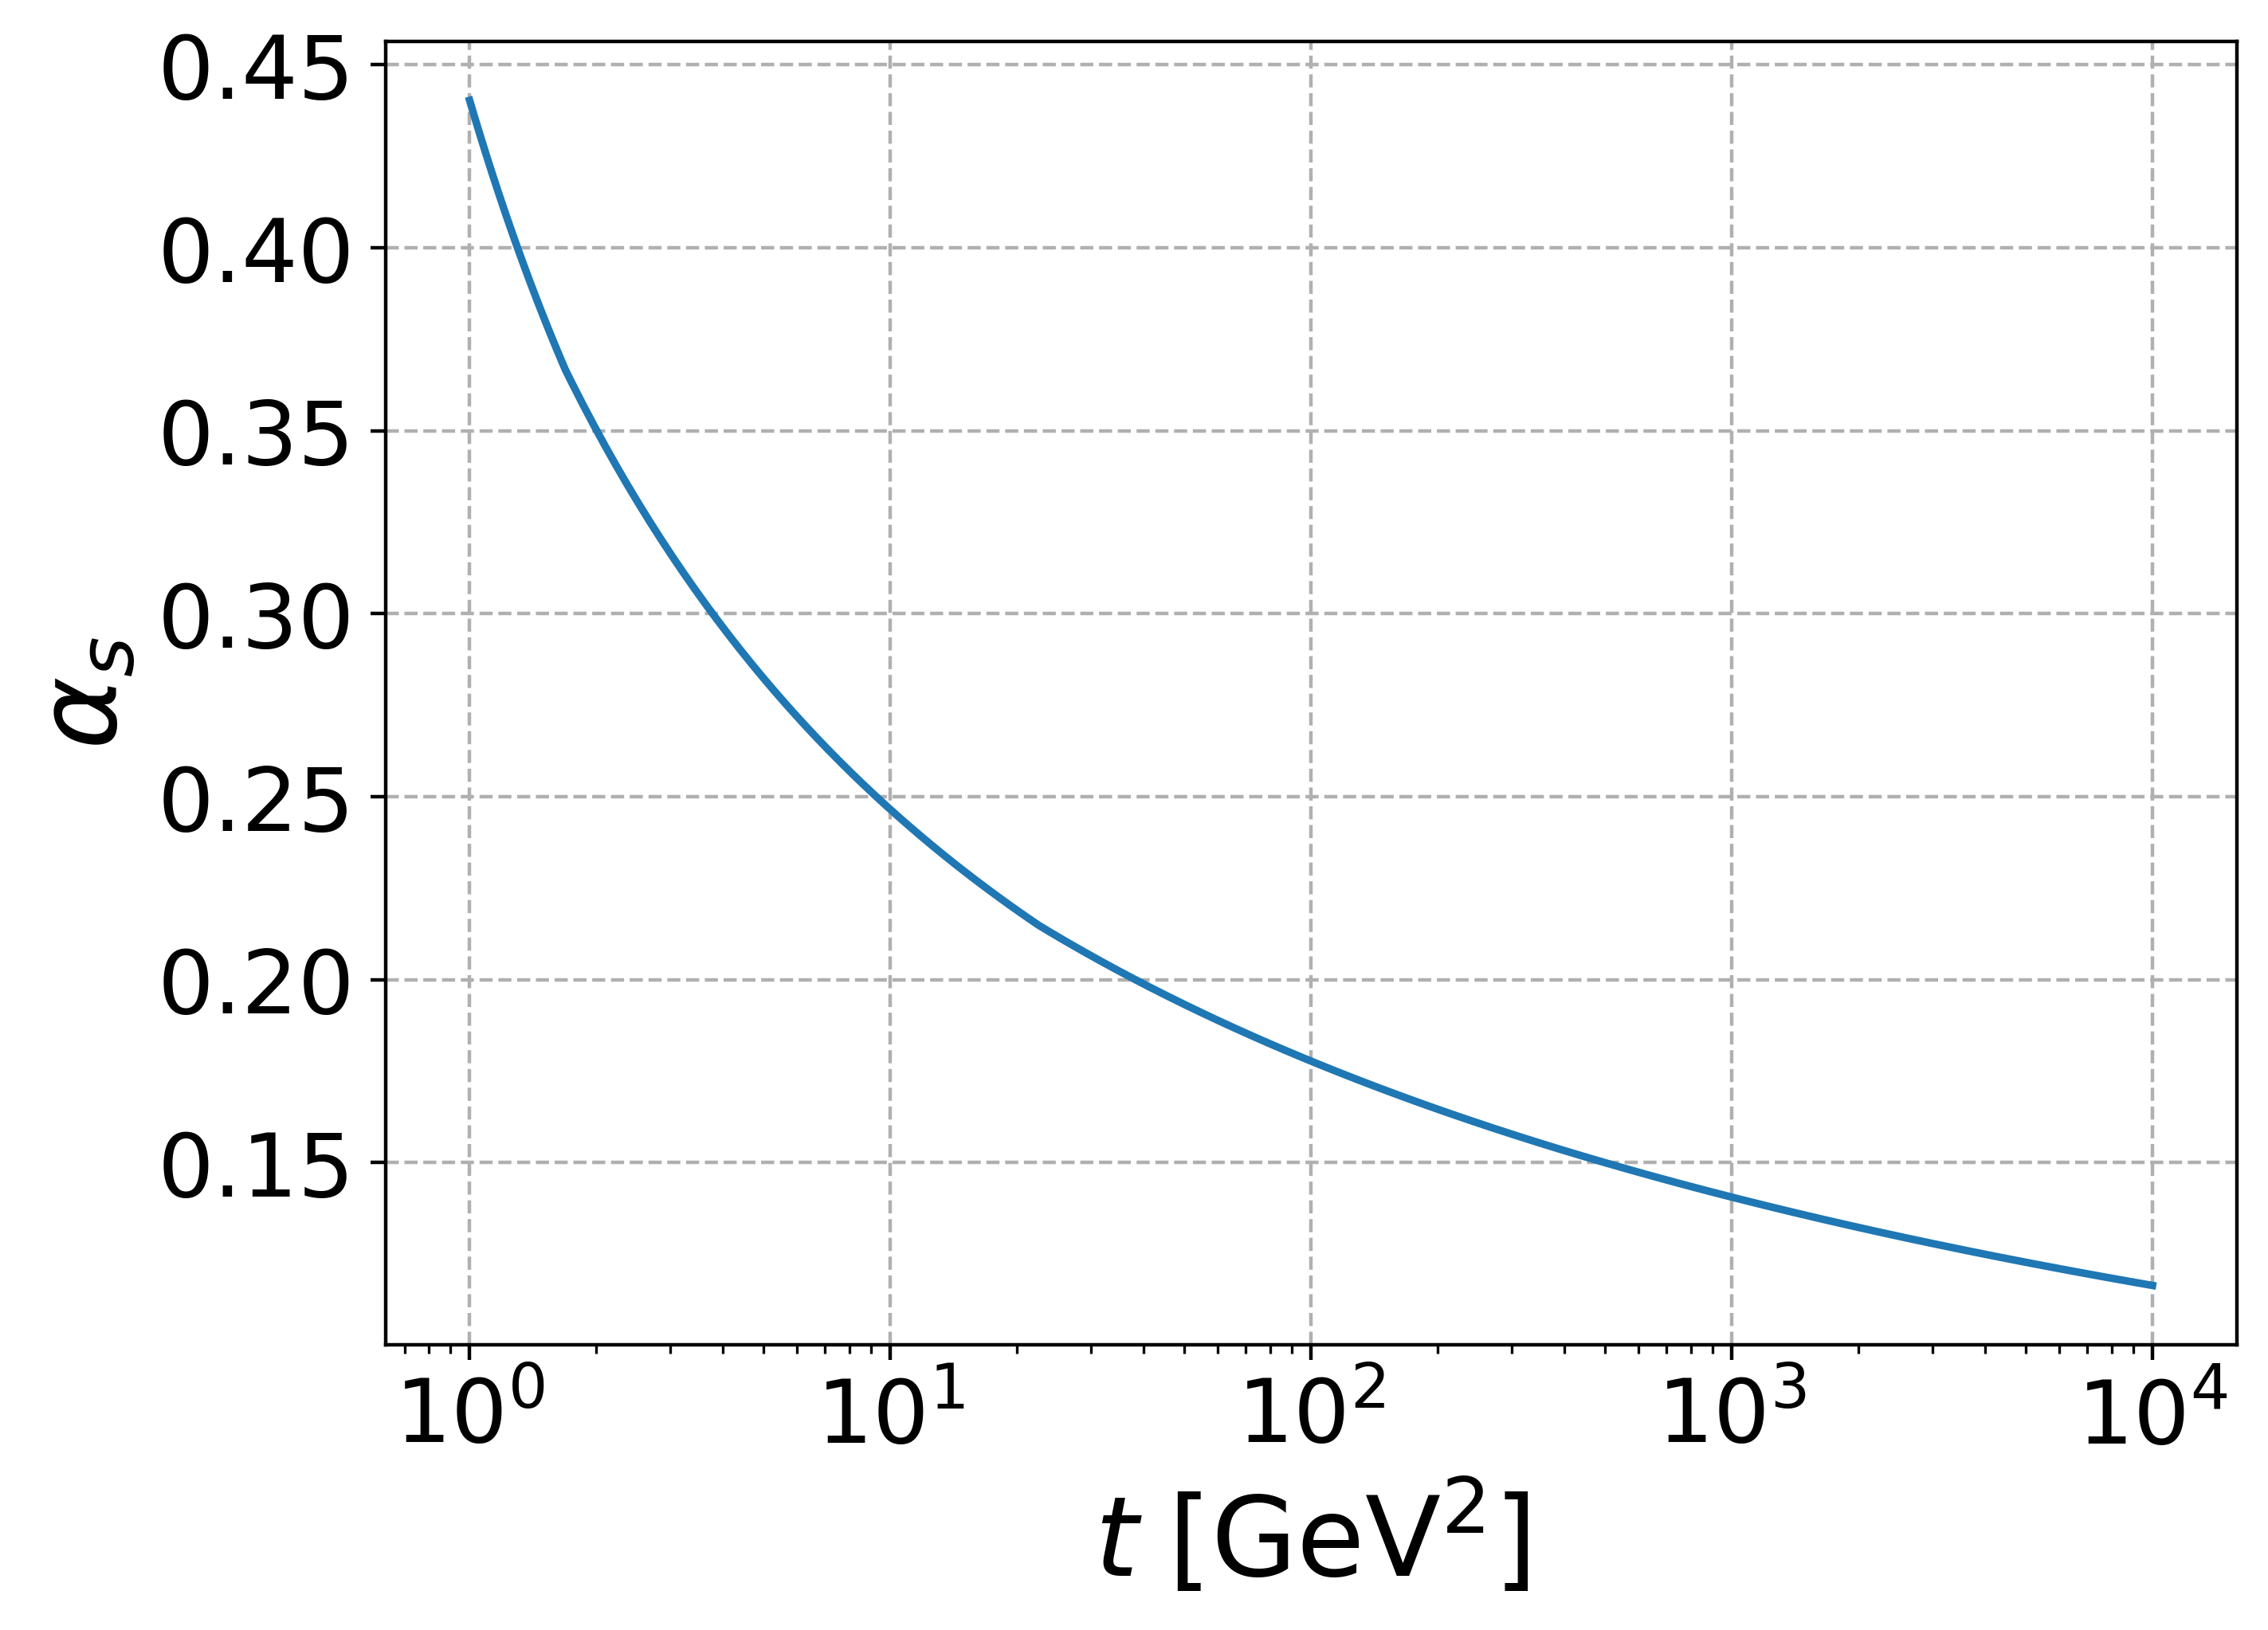
\includegraphics[width=0.5\textwidth]{figures/exercise2a.png}
  \caption{QCD coupling as a function of the squared energy scale.}
  \label{fig:2-alpha}
\end{wrapfigure}
This interaction between quarks and gluons is determined by the QCD coupling, $\alpha_{s}$, which, unlike the QED one, \textit{increases with decreasing energy scale}, see \autoref{fig:2-alpha}.\marginpar{Part a).} This means that some care is needed when trying to implement perturbation theory: \emph{if the energy scales become too small, the terms in the perturbative series cease to be smaller with increasing order}. 

One way to still apply perturbation theory and include this bremsstrahlung in the simulation, is to study this cascade in the kinematic limit where the emitted parton (i.e. a gluon or quark) is either collinear with its mother parton and/or soft, in other words, either the emission angle is small or the daughter's energy is small. In such case, the cross-section factorises into a part without the emission (the 2 -> 2 process of the previous section) and a universal emission factor, the latter enabling to treat subsequent emissions as a Markov Chain process, the simulation of which is called a “parton shower”. Furthermore, the restriction to small emission angles for the daughter particles gives rise to cone-shaped cascades, commonly referred to as \textit{partonic jets}.

\subsection{Monte Carlo integrator with parton shower}

Although the Monte Carlo integrator was developed from scratch, a \texttt{Shower} python class was provided for this project, the task being simply to “connect it” to the integrator.

An instance of \texttt{Shower} requires, for initialization, an instance of the class \texttt{AlphaS} and a lower cut-off scale $t_{0}$ (in $\text{GeV}^{2}$). The former is used to keep track of the “running” of the coupling $\alpha_{s}$ at different energy scales, while the latter represents a squared energy scale at which the emissions will be stopped when running the shower. Having created a single instance of it, the shower can be run with two arguments: (i) an \texttt{event}, consisting on a list of the incoming and outgoing particles, and (ii) the initial squared energy scale $t$. Then, the shower runs from the initial scale $t$ by generating emissions which lower the scale and modify in-place the \texttt{event} list (i.e. adds more particles to it), until the energy scale is below the cutoff, at which point the running stops.

The Monte Carlo integrator, being responsible for the cross-section factor without the emission, is precisely what is used to create the initial \texttt{event} list of particles. Each Monte Carlo point for the integrator has definite values of $s$, $\cos{\theta}$, $\phi$ and, performing a random sum over quark flavours, also a definite flavour q. From the kinematic variables, the momenta of the initial (electron-positron) and final particles (quark-antiquark) can be set, in the centre-of-mass frame, according to
\begin{equation}
    \begin{aligned}
        p_{\mathrm{e}^{-}} & = \frac{\sqrt{s}}{2} (1, 0, 0, -1), & \qquad p_{\mathrm{q}} & = \frac{\sqrt{s}}{2} (1, -\sin{\theta} \cos{\phi}, - \sin{\theta}\sin{\phi}, - \cos{\theta}) \\
        p_{\mathrm{e}^{+}} & = \frac{\sqrt{s}}{2} (1, 0, 0, +1), & \qquad p_{\bar{\mathrm{q}}} & = \frac{\sqrt{s}}{2} (1, +\sin{\theta} \cos{\phi}, + \sin{\theta}\sin{\phi}, + \cos{\theta}).
    \end{aligned}
\end{equation}
Besides the information of the momenta, the colour content of each particle also needs to be specified: the electron and the positron are colourless particles, the quark carries some colour and the antiquark carries the corresponding anti-colour. All this information is used to create instances of the \texttt{Particle} class (another class provided for the project), which form the elements of the initial \texttt{event} list.

Hence, the algorithm for the parton shower consists of sampling $N$ Monte Carlo points with the integrator, using the information of the kinematic variables and quark flavour to create one \texttt{event} per Monte Carlo point, to then pass these events to the shower, which modifies each of them in-place to yield events with final-state particles in them.

Following the above algorithm, the Monte Carlo integrator for a fixed beam distribution at the mass of the Z boson ($f(s) = \delta(s - M_{\mathrm{Z}}^{2})$) was used to generate 1,000 Monte Carlo points, which corresponded to the same number of events for which the parton shower was run. The cutoff scale was set to $t_{0} = 1 \text{GeV}^{2}$ and the initial scale at $t = M_{\mathrm{Z}}^{2}$. For each of these events, the number of final-state particles was counted and weighted according to its Monte Carlo weight, giving a \marginpar{Part c).}\emph{weighted average of 5.25(6) particles}.

\subsection{Jets and the Durham algorithm}

In the initialization of the parton shower discussed in the previous section, one of the required parameters is the energy scale cutoff $t_{0}$, below which the perturbative method no longer applies and the running of the shower is stopped. This unphysical parameter is introduced because the probabilities to emit additional quark or gluons at small angles or small energies diverges. However, in doing so, quantities like the number of particles after showering are ill-defined, as they depend on the choice of cutoff. At the same time, actual experiments have a limited resolution, which gives the possibility that additional collinear or soft partons are emitted, with the experimental signature being left unchanged.

In order to address both of these issues, jet algorithms have been developed. These algorithms cluster particles into jets that are well-separated, allowing for well-defined comparisons between experimental data and theory calculations.

For clustering the particles, two generic types of algorithms are commonly used: (i) cone algorithms and (ii) sequential recombination algorithms. In this project, the jet algorithm implemented for the analysis of the final state is the \textit{Durham $k_{T}$ algorithm}, which is of the second kind. This (final state) jet finding algorithm consists of the following:
\begin{enumerate}
    \item For each pair $(i, j)$ of final-state particles, compute the distance measure
    \begin{equation}
        y_{i j} = \frac{2 \text{min}(E_{i}^{2}, E_{j}^{2}) (1 - \cos{\theta_{ij}})}{Q^{2}},
    \end{equation}
    where $E_{i}$ is the energy of the $i$-th particle, $\theta_{i j} = \langle \mathbf{p}_{i}, \mathbf{p}_{j} \rangle$ is the angle between the spatial momenta, and $Q^{2}$ is a reference scale which, for this project, corresponds to the squared mass of the Z boson.

    \item Determine the pair of particles $(i, j)$ with the minimum $y_{i j}$ and combine them, i.e., sum their (four-)momenta.

    \item Repeat until all final-state particles are clustered into jets.
\end{enumerate}
The result of the above algorithm is a series of splitting scales, corresponding to the minimum values $y_{i j}$ found at each iteration. These splitting scales can then be used to quantify the contributions to the cross-section from different numbers of jets.

After implementing the Durham $k_{T}$ algorithm to cluster the final-state particles, an analysis of 1 million of events was carried out: The events were created using the Monte Carlo integrator at fixed beam energy, $s = M_{Z}^{2}$, for obtaining the initial and final-state particles properties, such as momentum and quark flavour, together with the Monte Carlo weights for each differential cross-section. The parton shower was then run for each of these events with a cutoff scale of $t_{0} = 1 \,\text{GeV}^{2}$ and an initial scale $t = M_{Z}^{2}$. The results can be seen in \autoref{fig:jet1} and \autoref{fig:jets}, where the results of the simulator are compared to those of \textsc{Sherpa} for differentials from 2 $\to$ 3 up to $5 \to 6$.

\begin{figure}[ht!]
    \centering
    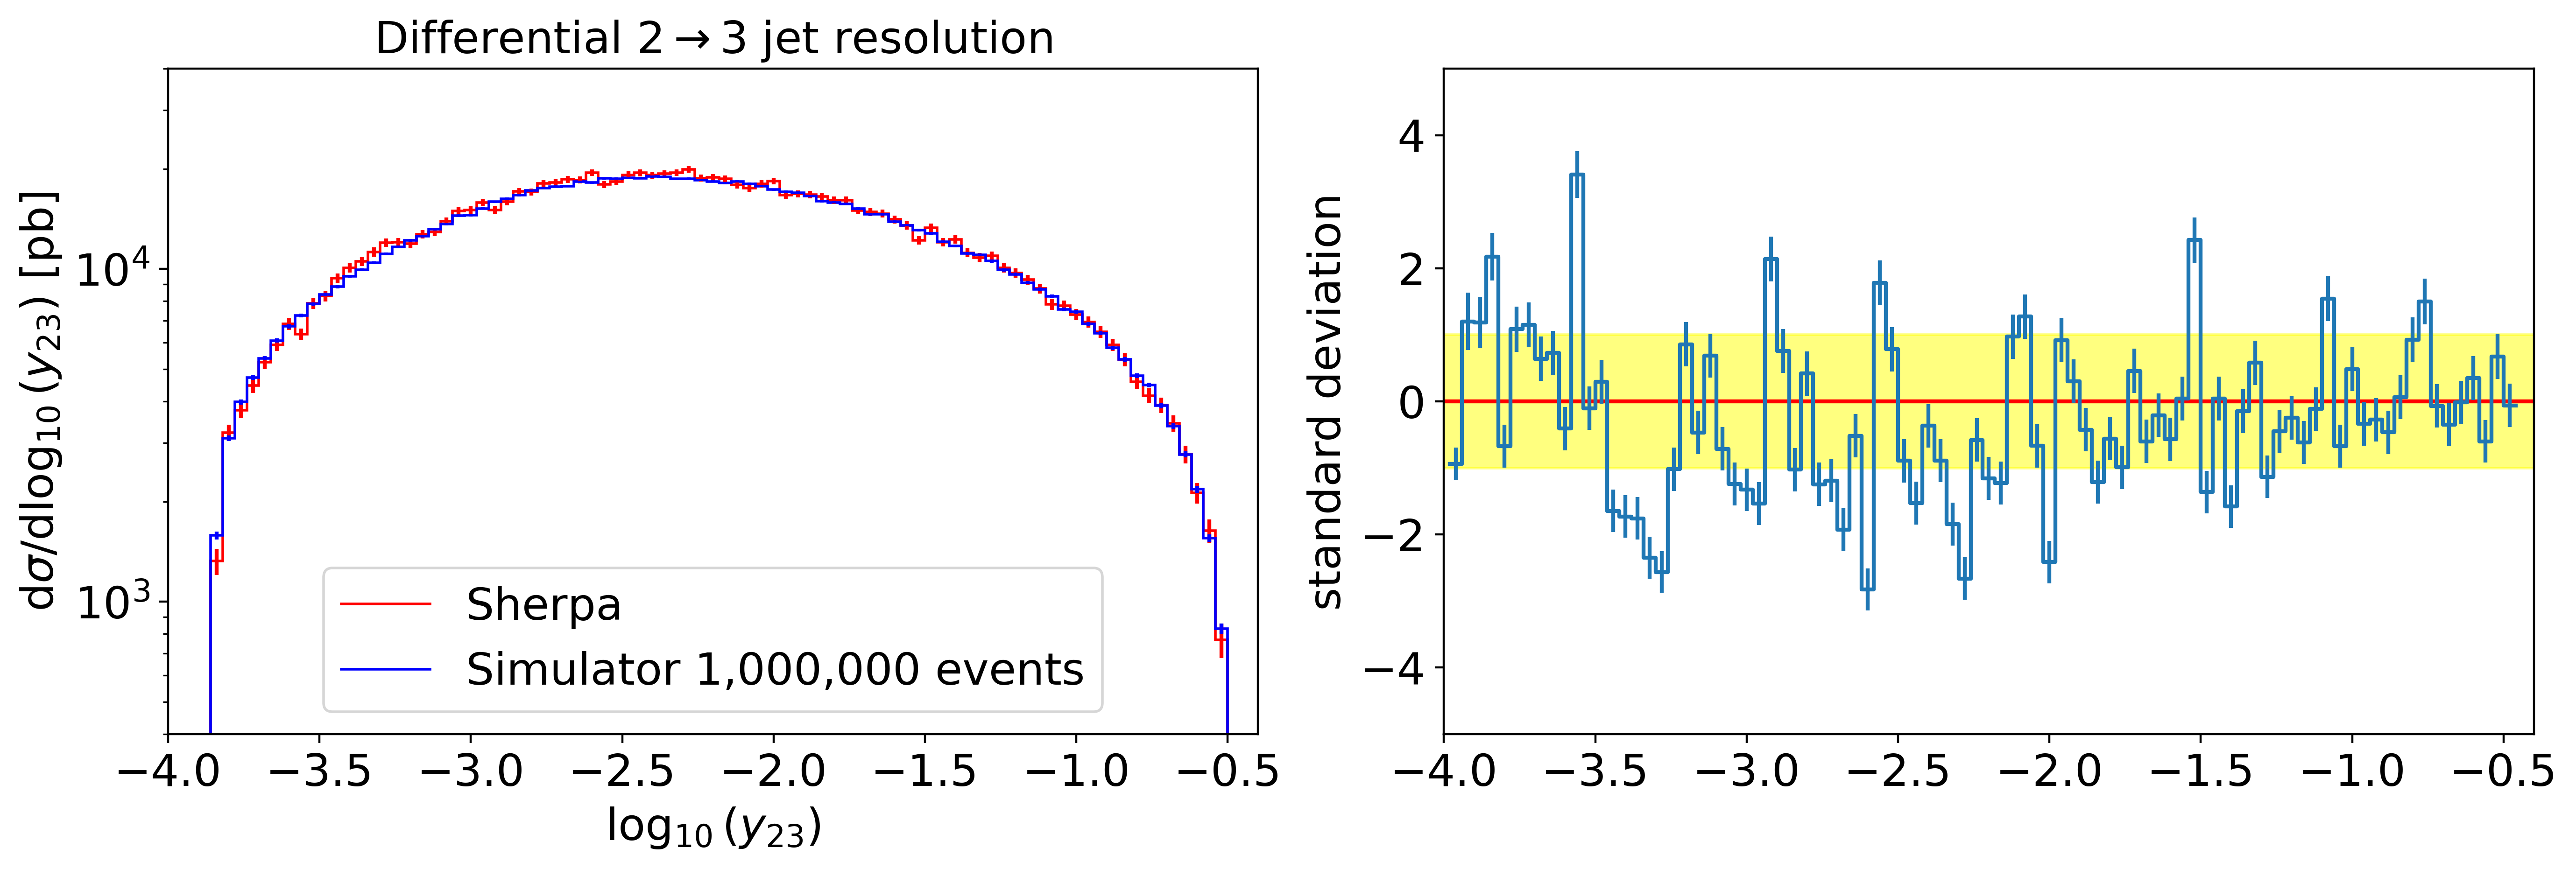
\includegraphics[width=\textwidth]{figures/jet_histo_1.png}
    \caption{}
    \label{fig:jet1}
\end{figure}

\clearpage

\begin{figure}[ht!]
    \centering
    \begin{subfigure}[t]{\textwidth}
        \centering
        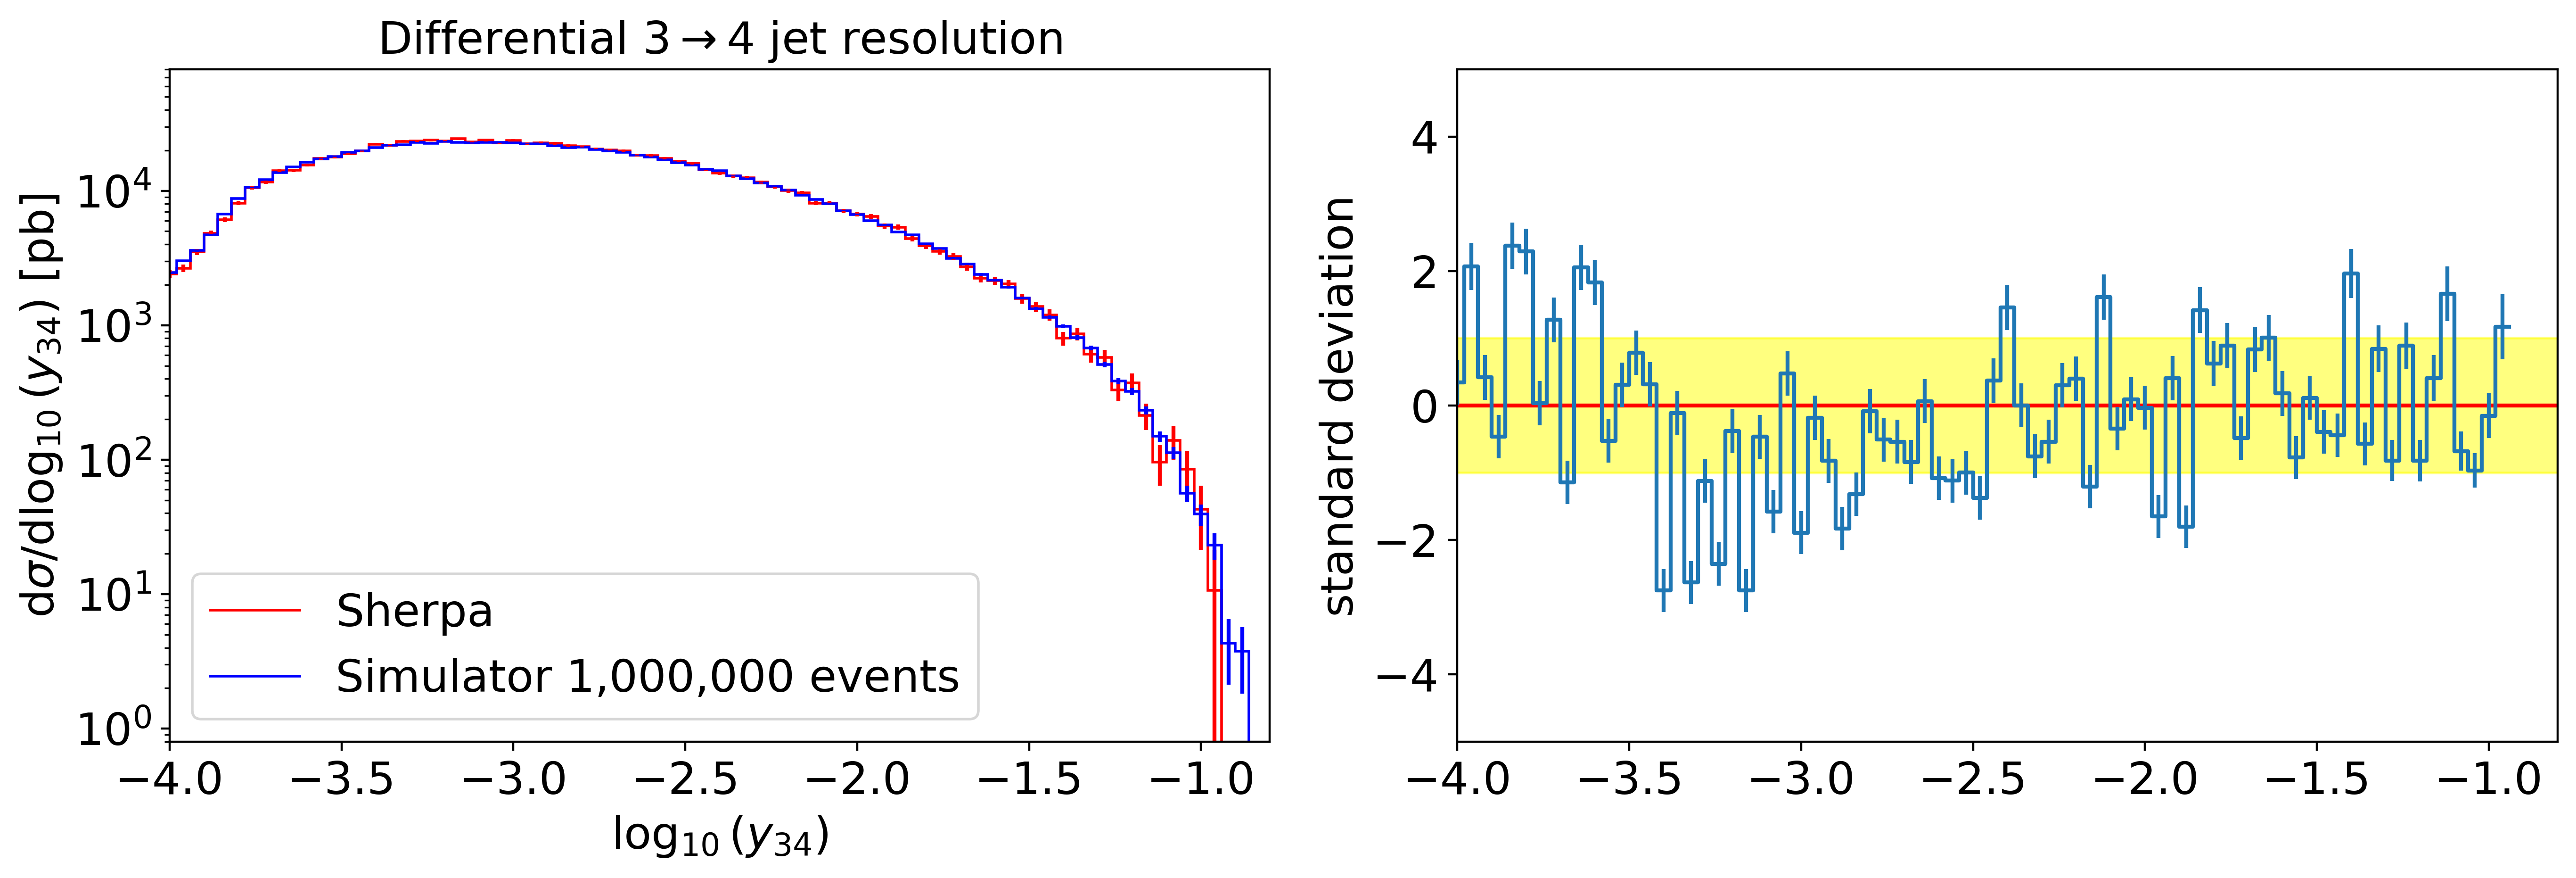
\includegraphics[width=\textwidth]{figures/jet_histo_2.png}
        \caption{}
        \label{fig:jet2}
    \end{subfigure}
    \hfill
    \begin{subfigure}[t]{\textwidth}
        \centering
        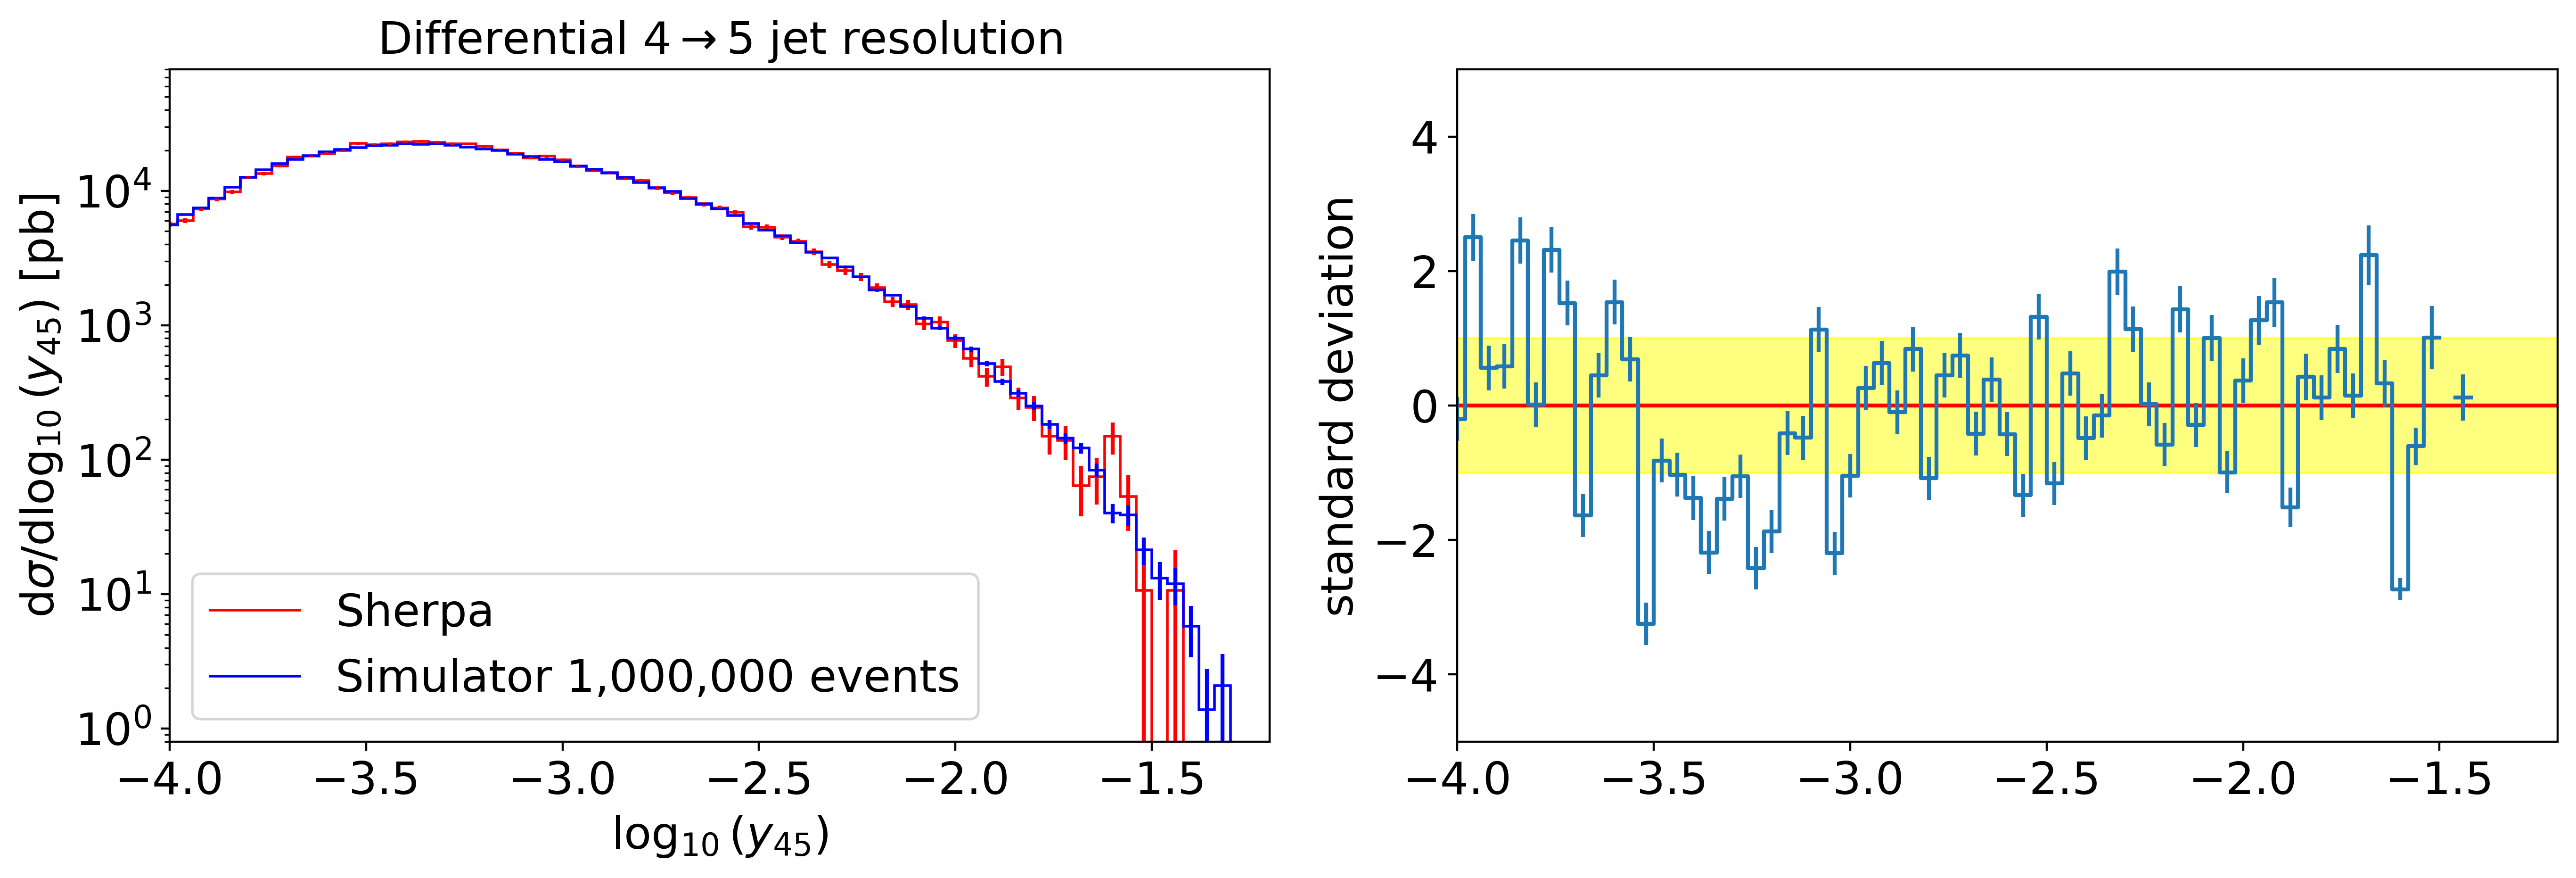
\includegraphics[width=\textwidth]{figures/jet_histo_3.png}
        \caption{}
        \label{fig:jet3}
    \end{subfigure}
    \hfill
    \begin{subfigure}[t]{\textwidth}
        \centering
        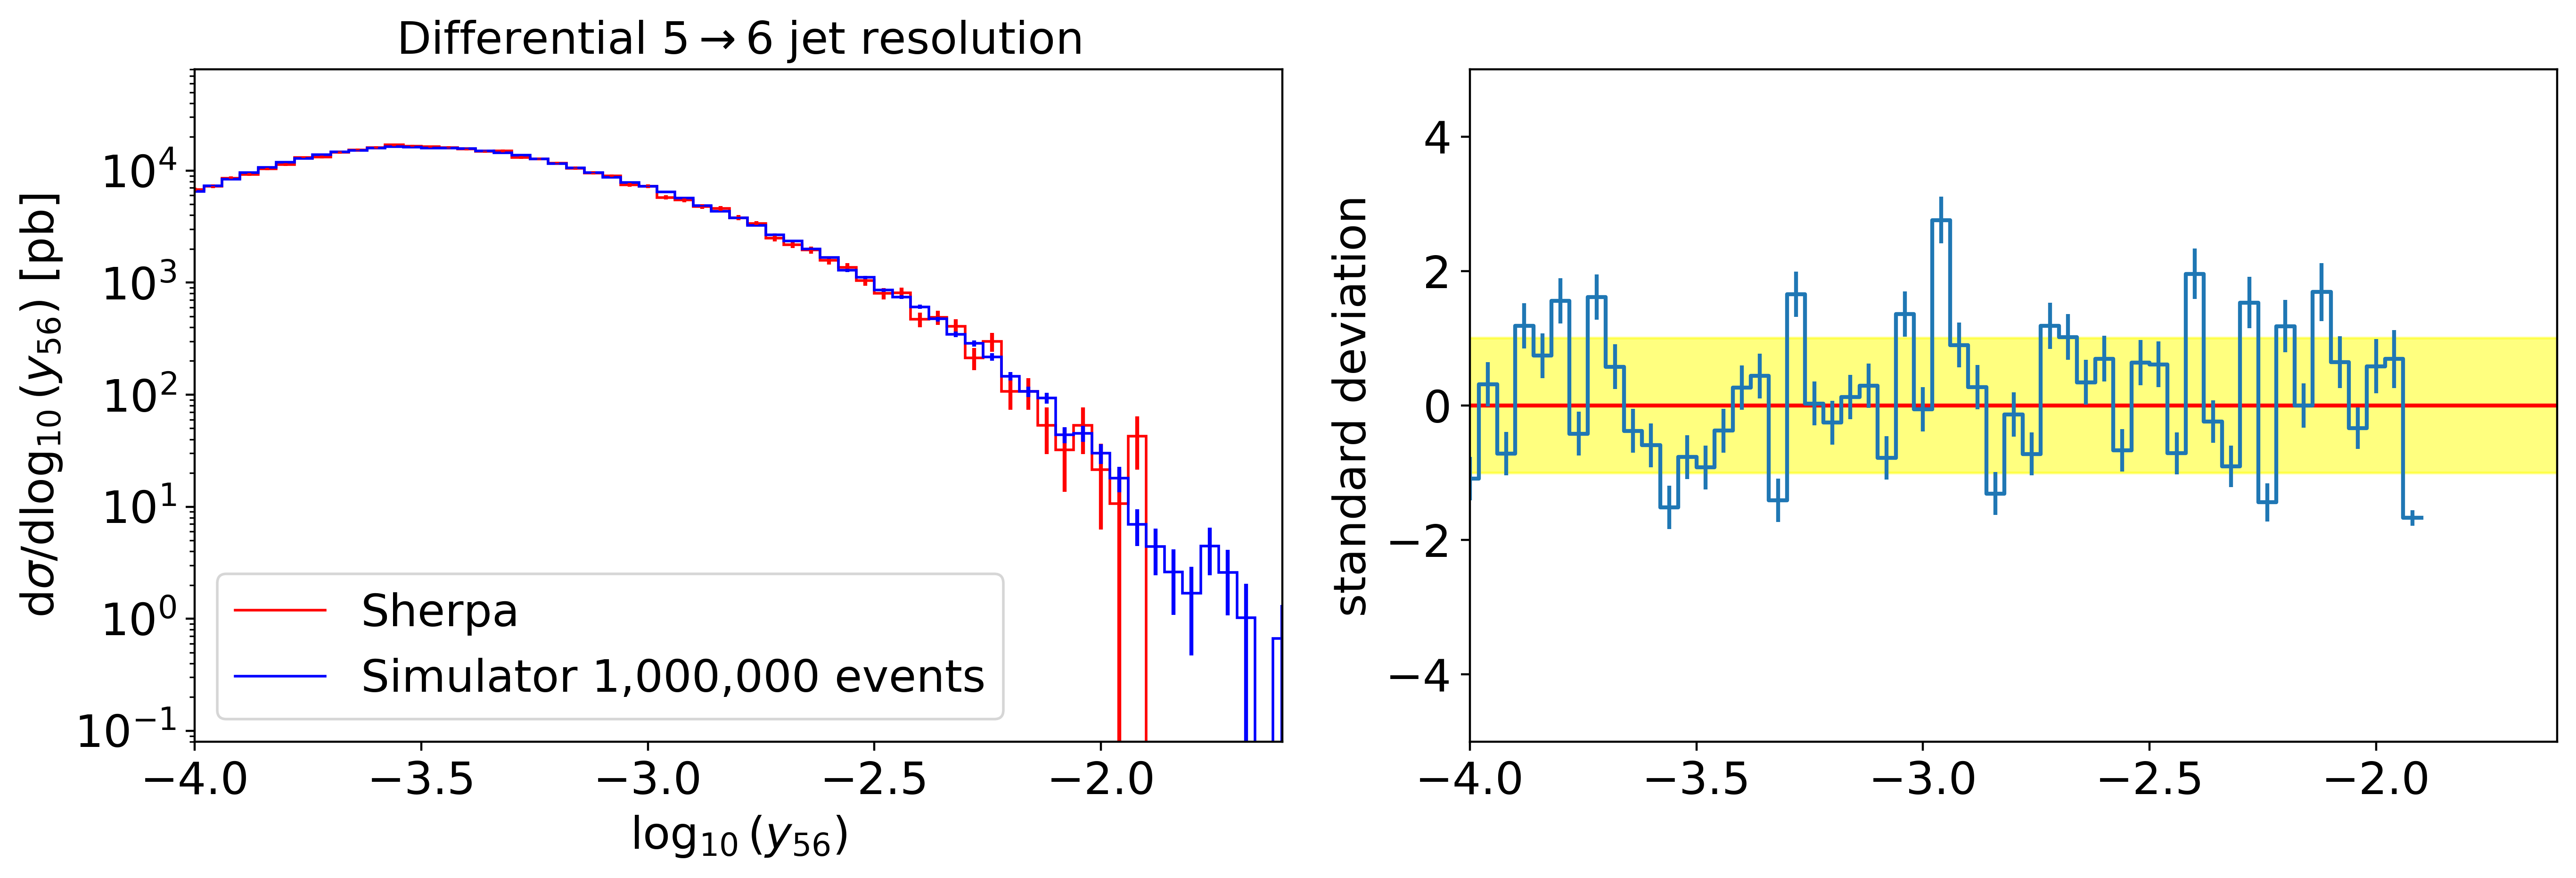
\includegraphics[width=\textwidth]{figures/jet_histo_4.png}
        \caption{}
        \label{fig:jet4}
    \end{subfigure}
    \caption{Jet resolution for several differentials. The plots on the right are the associated errors, in standard deviations, to the values of \textsc{Sherpa}.}
    \label{fig:jets}
\end{figure}

\begin{appendix}
    \section{Numerical values and squared matrix element} \label{sec:app-num-values}

The physical constants used throughout the project are given in \autoref{tab:app-num-constants}.
\begin{table}[ht!]
    \centering
    \renewcommand{\arraystretch}{1.3}
    \setlength{\arrayrulewidth}{0.3mm}
    \begin{tabular}{ccl}
        \hline Symbol & Value & Description \\ \hline
        $\alpha$ & 1/129 & QED coupling \\
        $\alpha_{s}(M_{\text{Z}})$ & 0.118 & QCD coupling at the Z mass scale \\
        $M_{\text{Z}}$ & 91.2 & Z boson mass \\
        $\Gamma_{\text{Z}}$ & 2.5 & Z boson decay width \\
        $\sin^{2}{\theta_{W}}$ & 0.223 & squared sine of the Weinberg angle \\
        $Q_{\text{e}}$ & -1 & electric charge of the electron \\
        $Q_{\text{u,c}}$ & 2/3 & electric charge of (light) up-type quarks \\
        $Q_{\text{d,s,b}}$ & -1/3 & electric charge of down-type quark \\
        $T^{3}_{\text{u,c}}$ & 1/2 & weak isospin of (light) up-type quarks \\
        $T^{3}_{\text{d,s,b,e}}$ & -1/2 & weak isospin of down-type quarks and the electron \\
        $N_{q}$ & 5 & number of light quark flavours (i.e. u, d, s, c, and b) \\
        $N_{C}$ & 3 & number of QCD colours \\
        $f_{\text{conv}}$ & 3.89379656 $\cdot 10^{8}$ & physical units conversion factor \\ \hline
    \end{tabular}
    \caption{Numerical constants used throughout the project. Masses and decay widths are given in GeV.}
    \label{tab:app-num-constants}
\end{table}

To leading order, the squared matrix element for the process $\mathrm{e}^{-} \mathrm{e}^{+} \to \mathrm{q} \bar{\mathrm{q}}$ is given by
\begin{equation}
    \begin{aligned}
    \lvert \mathcal{M}_{\mathrm{q} \bar{\mathrm{q}}} \rvert^{2} = (4 \pi \alpha)^{2} N_{C} & \left[
    \left( 1 + \cos^{2}{\theta} \right) \left\{ Q_{\mathrm{e}}^{2} Q_{\mathrm{q}}^{2} + 2 Q_{\mathrm{e}} Q_{\mathrm{q}} V_{\mathrm{e}} V_{\mathrm{q}} \chi_{1}(s) + \left( A_{\mathrm{e}}^{2} + V_{\mathrm{e}}^{2} \right) \left( A_{\mathrm{q}}^{2} + V_{\mathrm{q}}^{2} \right) \chi_{2}(s) \right\}
    \right. \\
    & \left. \qquad + \cos{\theta} \left\{ 4 Q_{\mathrm{e}} Q_{\mathrm{q}} A_{\mathrm{e}} A_{\mathrm{q}} \chi_{1}(s) + 8 A_{\mathrm{e}} V_{\mathrm{e}} A_{\mathrm{q}} V_{\mathrm{q}} \chi_{2}(s) \right\} \right],
    \end{aligned}
\end{equation}
where
\begin{equation}
    V_{\mathrm{f}} = T_{\mathrm{f}}^{3} - 2 Q_{\mathrm{f}} \sin^{2}{\theta_{W}} \qquad \text{and} \qquad A_{\mathrm{f}} = T_{\mathrm{f}}^{3}
\end{equation}
are the vector and axial couplings of the fermions to the Z boson, respectively, and 
\begin{equation}
    \chi_{1}(s) = \frac{ \kappa s (s - M_{\text{Z}}^{2})}{(s - M_{\text{Z}}^{2})^{2} + \Gamma_{\text{Z}}^{2} M_{\text{Z}}^{2}}, \quad \chi_{2}(s) = \frac{\kappa^{2} s^{2}}{(s - M_{\text{Z}}^{2})^{2} + \Gamma_{\text{Z}}^{2} M_{\text{Z}}^{2}}, \quad \kappa = \frac{1}{4 \sin^{2}{\theta_{W}}(1 - \sin^{2}{\theta_{W}})}.
\end{equation}

    \section{Integration grids generated by Vegas} \label{sec:app-int-grids}

The adaptive algorithm implemented in the \texttt{vegas} package approximates the distributions for each integration variable to improve the evaluations of the integral. From these distributions, different grids for pairs of integration variables can be shown, helping to understand for which points in phase space do higher contributions to the integral occur. The first of these integration grids was shown in \autoref{fig:ex1e_one_grid}, corresponding to the pair of kinematic variables $s$ and $\cos{\theta}$. Since the integrand depends only on these two variables, it is arguably the most insightful one. Here, however, the other two integration grids are shown in \autoref{fig:app-integration-grids} for completeness, as they allow to confirm that \texttt{vegas} did find a uniform distribution along $\phi$. Furthermore, these two integration grids also display more clearly the higher contributions of $s$ for values closer to $M_{\text{Z}}^{2}$, the mass of the Z boson, as well as the asymmetrical contributions for $\cos{\theta}$ towards $+1$ and $-1$, the distribution being slightly more dense towards 1.

\begin{figure}[ht!]
     \centering
     \begin{subfigure}[t]{0.49\textwidth}
         \centering
         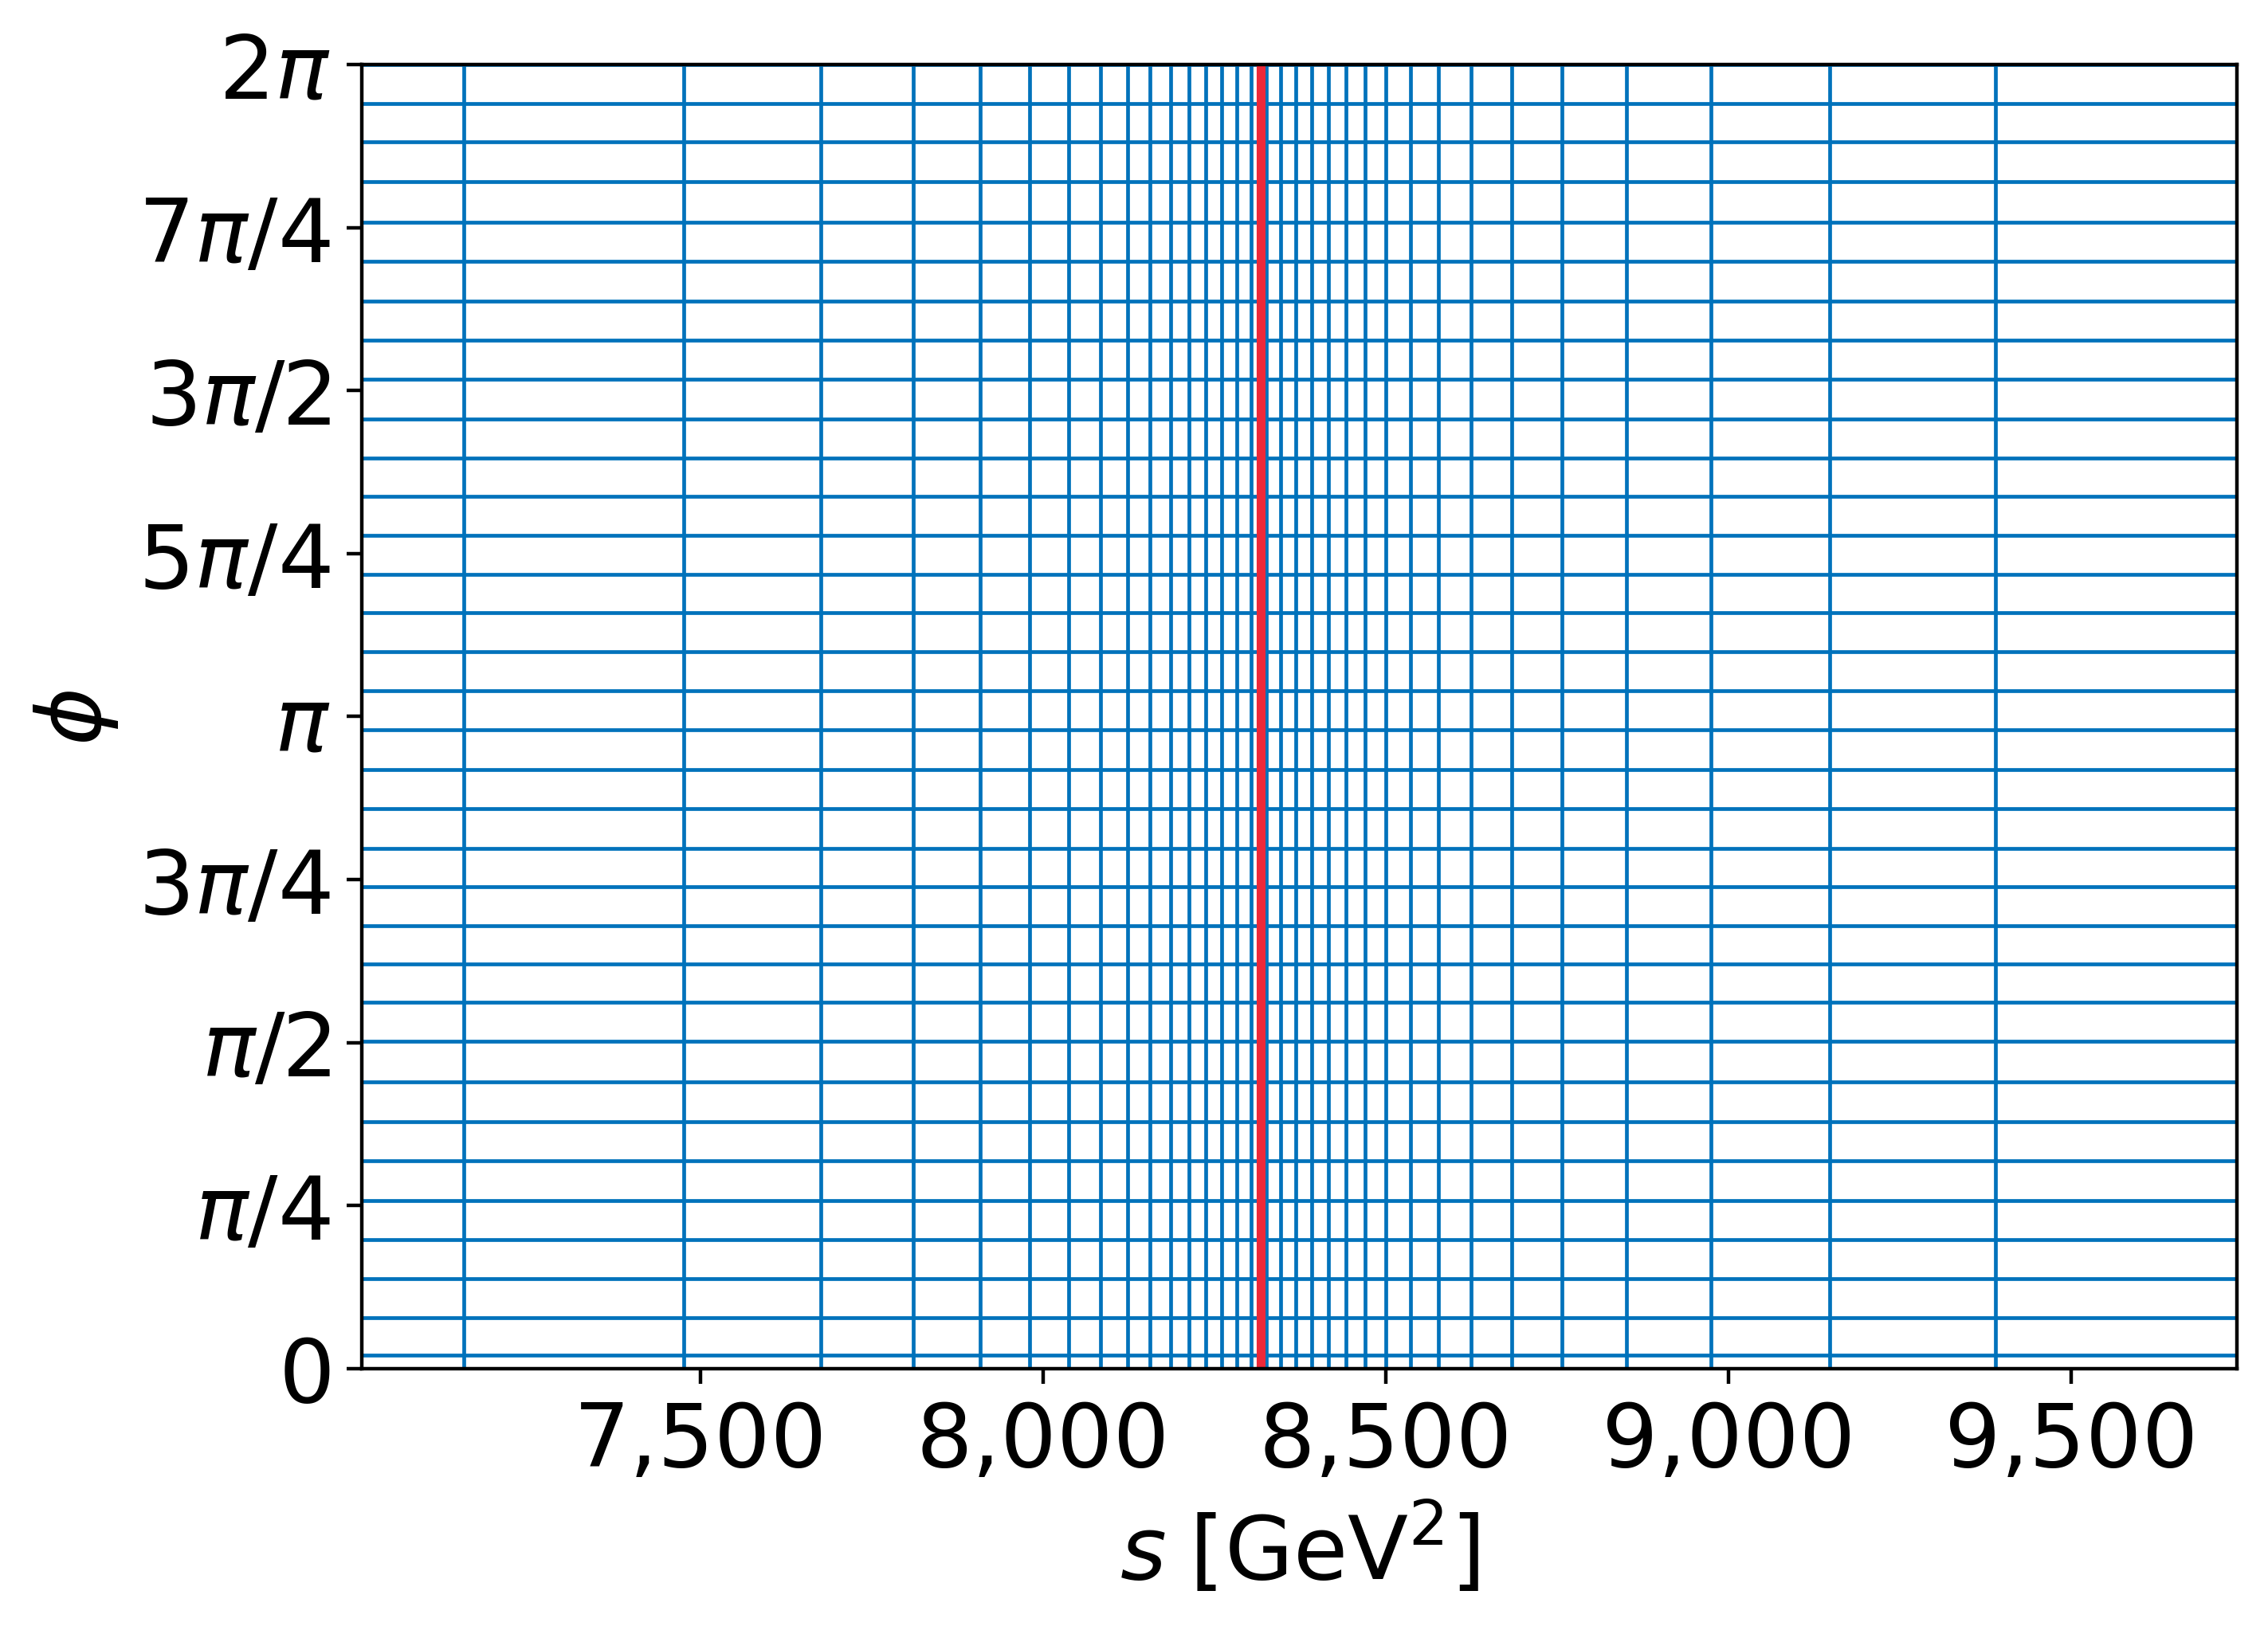
\includegraphics[width=\textwidth]{figures/integration_grid_1.png}
         \caption{}
         \label{fig:app-integration-grid1}
     \end{subfigure}
     \hfill
     \begin{subfigure}[t]{0.49\textwidth}
         \centering
         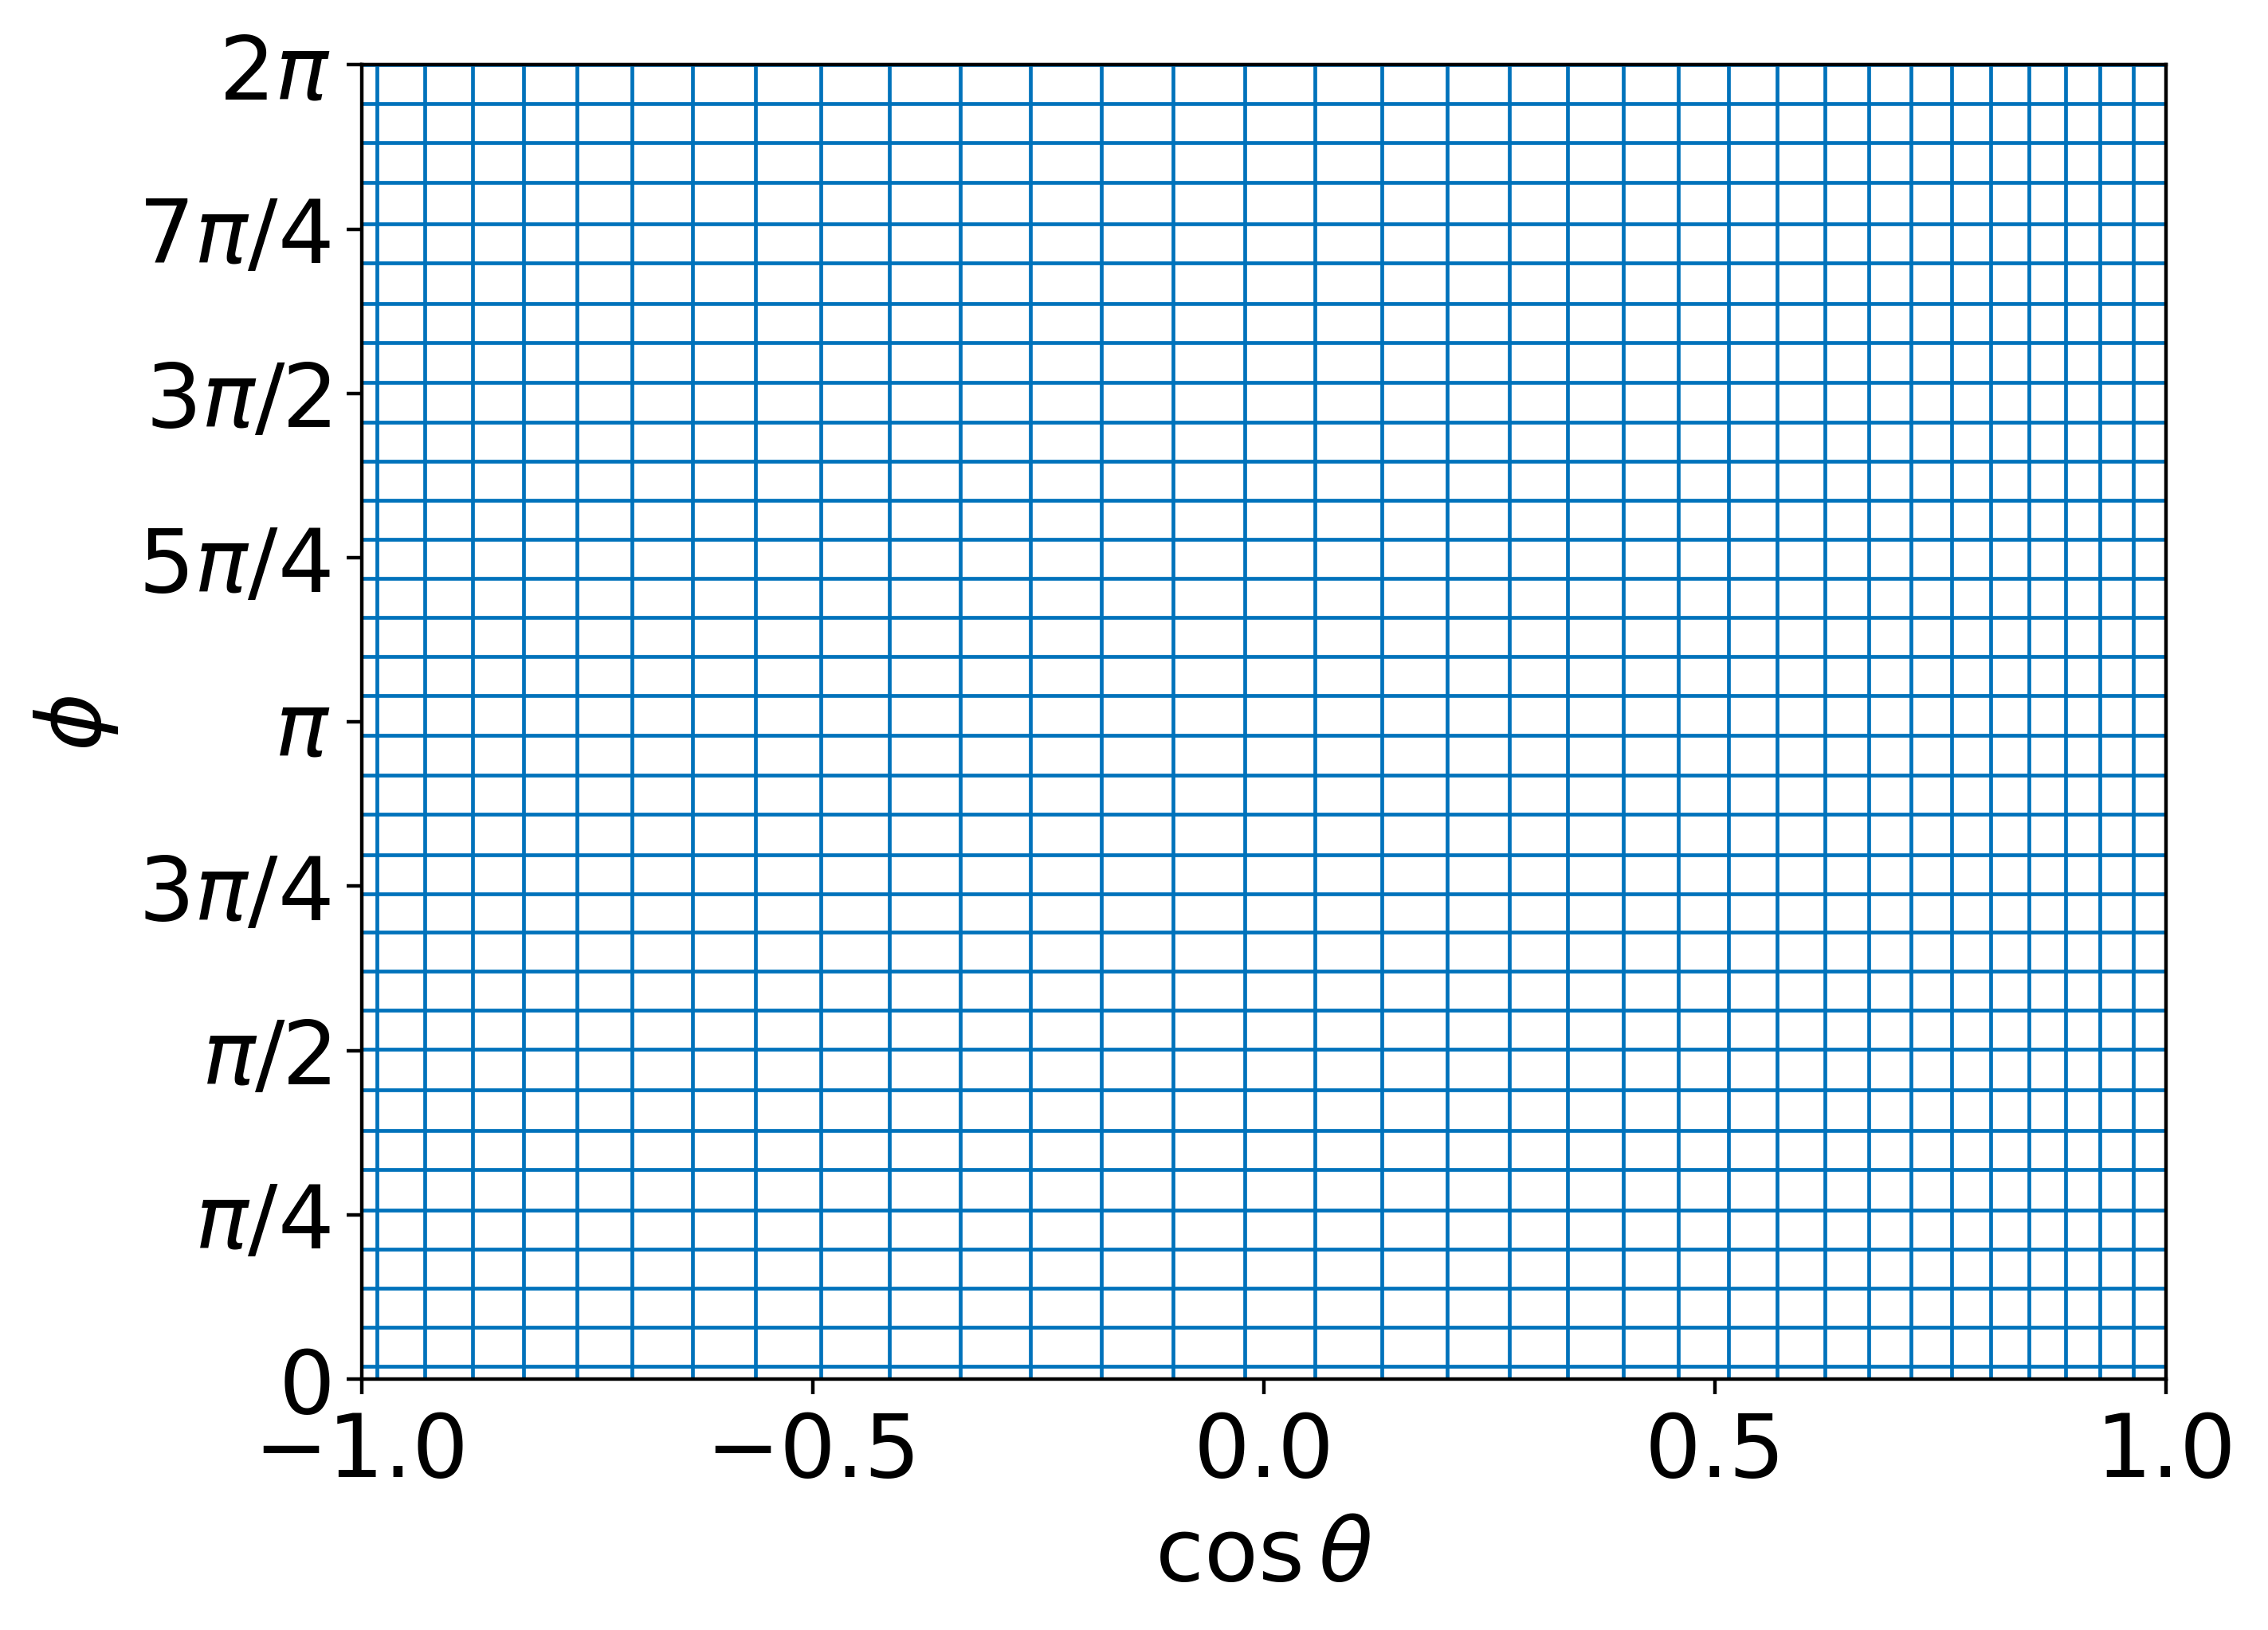
\includegraphics[width=\textwidth]{figures/integration_grid_2.png}
         \caption{}
         \label{fig:app-integration-grid2}
     \end{subfigure}
        \caption{Vegas integration grids for the other two pairs of kinematic variables. The red line corresponds to $s = M_{Z}^{2}$.}
        \label{fig:app-integration-grids}
\end{figure}

\end{appendix}

\end{document}
